% !Mode:: "TeX:UTF-8"
\documentclass[type=profmaster,openany,pifootnote]{shuthesis}
% 选项:
%  type=[master|profmaster|doctor], % 必选
%  secret,                          % 可选 (如果论文需要保密, 这一项需要打开)
%  pifootnote,                      % 可选（建议打开）
%  openany|openright,               % 可选 (章首页是右开还是任意开, 默认是右开)
%  nocolor                          % 提交最终版本时请打开此选项
\usepackage{shuthesis}
\usepackage{bm}
\usepackage{titlesec}
\usepackage{fontspec}
% \setmonofont{Courier New} 
\setmonofont{Ubuntu Mono}
\graphicspath{{figures/}}

\renewcommand{\thesubsubsection}{\arabic{subsubsection}）}
\titleformat{\subsubsection}[block]
  {\normalfont\bfseries} % 字体样式：常规字体，加粗
  {\thesubsubsection}    % 标题编号
  {0.5em}                % 编号与标题文字之间的间距
  {}                     % 标题文字前的特殊代码

% \titlespacing{命令}{左间距}{上间距}{下间距}
\titlespacing{\subsubsection}{0pt}{1.0ex plus .1ex minus .2ex}{0.5ex plus .1ex}


\begin{document}
\frontmatter
\shusetup{
  %%%%%%%% 1. 配置里面不要出现空行. 2. 不需要的配置信息可以删除. %%%%%%%%%%%
  secretlevel={公开},             % 秘级
  % 中文信息
  ctitle={基于学习的点云几何特征检测及机器人抓取规划方法研究},
  cdisciplines={工学},
  cdepartment={机电工程与自动化学院},
  cmajor={机械},
  cauthor={邱模聪},
  csupervisor={袁建军},
  id={23722063},
  catalognumber={XXX},
  cdate={2026 年 5 月},
  coverdate={\zhdigits{2026}年\zhnumber{5}月},
  % 英文信息
  etitle={Learning-Based Point Cloud Geometric Feature Detection and Robotic Grasp Planning},
  edisciplines={Engineering},
  edepartment={School of Mechatronic Engineering and Automation},
  emajor={Mechanics},
  eauthor={Mocong Qiu},
  esupervisor={Jianjun Yuan},
  edate={December, 2026}
}

% 中英文摘要和关键字
\begin{cabstract}
针对物体几何特征检测精度不足及机器人抓取规划灵活性受限的问题，本文提出一种融合神经网络特征学习与基于模型进行机器人抓取规划的框架。首先，本文提出基于多维特征融合的点云边缘角点检测网络（NECDNet）。该网络通过分析点云多尺度邻域内的位置和法向分布构建特征矩阵，利用层次化神经网络实现面、边、角点的同步分类，提取物体几何特征；同时构建了包含1000个模型的ABC-Corner数据集用于网络训练。其次，本文提出一种考虑边、角接触的六自由度双指抓取规划算法。该算法利用NECDNet提取特征区域，设计特征化接触检测器搜索对偶接触点，并引入软接触模型评估稳定性，有效解决了非规则物体的抓取难题，增强抓取规划多样性。实验表明，NECDNet的角点检测F1分数达0.815，优于现有方法；机器人抓取规划算法在分布复杂度指标（STD、Range、MAD）均优于GPD，GraspIt等基于模型的抓取规划方法，抓取构型灵活性显著提升。机器人实验验证了包括角-角、角-边等六种接触组合的有效性与鲁棒性，展示了抓取规划的有效性及抓取成功率上的提升。
\end{cabstract}

\ckeywords{点云处理, 几何特征检测, 神经网络, 机器人抓取规划, 二指平行手爪}

\begin{eabstract}
To address the limited accuracy of object geometric feature detection and the restricted flexibility of robotic grasp planning, this thesis proposes a framework that combines neural-network feature learning with model-based robotic grasp planning. First, a multi-feature fusion point-cloud edge and corner detection network, NECDNet, is developed. NECDNet builds feature matrices from positional and normal distributions in multi-scale neighborhoods, and uses a hierarchical neural architecture to jointly classify faces, edges, and corners for geometric feature extraction. In addition, the ABC-Corner dataset with 1,000 models is constructed for network training. Second, a six-degree-of-freedom two-finger grasp planning algorithm considering edge and corner contacts is proposed. Based on feature regions extracted by NECDNet, the algorithm designs feature-aware contact detectors to search for antipodal contact pairs, and introduces a soft-contact model for stability evaluation. This effectively addresses grasping challenges for irregular objects and improves the diversity of grasp planning. Experiments show that NECDNet achieves a corner-detection F1 score of 0.815, outperforming existing methods. The proposed grasp planning algorithm also outperforms model-based methods such as GPD and GraspIt on distribution complexity metrics (STD, Range, and MAD), with a significant gain in grasp configuration flexibility. Robotic experiments further verify the effectiveness and robustness of six contact combinations, including corner-corner and corner-edge contacts, demonstrating improved grasp planning performance and grasp success rate.
\end{eabstract}

\ekeywords{Point cloud processing, Geometric feature detection, Neural network, Robotic grasp planning, Two-finger parallel gripper}

\makefirstpage                         % 生成带有学校 logo 的封面
\makecover

\tableofcontents                       % 目录

% !Mode:: "TeX:UTF-8"
\begin{denotation}[2.5cm]
\item[$\mathcal{P}^\text{c}$] 非结构化点云
\item[$n$] 点云中点的数量
\item[$\mathbf{p}_i^\text{c}$] 查询点（点云中第 $i$ 个点的三维坐标）
\item[$\mathcal{Q}_i^\text{c}$] 查询点 $\mathbf{p}_i^\text{c}$ 的邻域点集合
\item[$k$] 查询点邻域 $\mathcal{Q}_i^\text{c}$ 中点的数量
\item[$\mathbf{n}_i^\text{c}$] 查询点 $\mathbf{p}_i^\text{c}$ 的法向量
\item[$\kappa_i$] 查询点邻域的曲率特征
\item[$\bar{d}_i$] 查询点邻域的投影距离均值特征
\item[$r_i$] 查询点邻域的中心偏离比特征
\item[$\mu_{\theta,i}$] 查询点邻域的法向量角度差均值特征
\item[$\sigma^2_{\theta,i}$] 查询点邻域的法向量分布方差特征
\item[$\bar{\text{proj}_i}$] 查询点邻域的法线投影距离均值特征
\item[$\mathbf{x}_i^\text{c}$] 查询点 $\mathbf{p}_i^\text{c}$ 在某一尺度下的局部特征向量
\item[$\mathbf{X}_i^\text{c}$] 查询点 $\mathbf{p}_i^\text{c}$ 的多尺度特征矩阵
\item[$m$] 多尺度特征矩阵中的尺度数量
\item[$\mathcal{S}$] 用于抓取规划的采样点集合
\item[$\mathbf{s}_i$] 采样点（集合 $\mathcal{S}$ 中第 $i$ 个点）
\item[$f_i$] 采样点 $\mathbf{s}_i$ 的几何特征类别标签
\item[$\mathtt{f}, \mathtt{e}, \mathtt{c}$] 几何特征类别：面点、边缘点、角点
\item[$v$] 体素采样尺寸参数
\item[$\mathcal{D}_i$] 基于几何特征的接触检测器
\item[$d$] 接触检测器（或机械手指腹）的直径
\item[$l$] 接触检测器的长度
\item[$\theta_{\mathrm{sec}}$] 边特征检测器（扇形柱）的张角
\item[$\theta_{\mathrm{cone}}$] 角特征检测器（圆锥体）的顶角
\item[$\theta_{\mathrm{th}}$] 对偶接触点法向对齐验证阈值
\item[$\mathbf{j}_i$] 机械手抓取中心位置
\item[$\mathbf{v}_i$] 机械手接触向量（接近方向）
\item[$\beta$] 机械手绕接触轴的旋转增强角度
\item[$\eta$] 软指腹有效压缩系数
\item[$\mathbf{C}_i$] 软接触模型下的离散接触点簇
\end{denotation}
                % 符号对照表

% 正文部分
\mainmatter
% !Mode:: "TeX:UTF-8"
\chapter{研究背景与意义}
\label{cha:intro}

\section{研究背景}
\label{sec:background}

随着智能制造、服务机器人以及自动驾驶技术的飞速发展，具备高精度环境感知与自主交互能力的智能系统正成为学术界与工业界的研究焦点。在这一领域中，三维点云（3D Point Clouds）凭借其对物体几何结构和空间尺度的精确表达能力，已成为连接物理世界与数字世界的重要纽带。作为一种无序、非结构化的数据集合，点云能够直接反映物体的真实拓扑结构，不存在二维图像中的透视形变，因此被广泛应用于逆向工程、三维重建、场景理解以及机器人自主抓取等关键任务中~\cite{mirzaei_3d_2022}。

在点云数据分析中，物体几何特征（尤其是边缘与角点）的提取不仅是数据简化的过程，更是语义理解的关键。边缘勾勒了物体的轮廓骨架，角点则确立了形体的关键节点。这些特征承载了最丰富的结构语义信息：在三维重建中，它们往往作为曲面拟合的自然边界，决定了重建模型的保真度~\cite{li_surface_2023}；在物体识别与配准任务中，它们充当了具有高辨识度的关键描述符，能够显著提升算法在复杂场景下的鲁棒性~\cite{lavin-delgado_efficient_2024, GaoJunJie_ji_2024, ZhangZhiJia_ji_2017}；而在机器人操作领域，准确的轮廓信息更是实现精细化装配与灵巧抓取的前提条件~\cite{ahmed_edge_2018}。

尽管物体几何特征具有重要的应用价值，但从非结构化点云中自动且精确地检测这些特征仍面临严峻挑战。首先受限于物理平滑及采样精度，现实物体原本的尖锐几何特征在点云数据中往往表现为一定范围内的圆角过渡区域，使得边缘和角点的界定变得模糊，不利于检测。其次是不同类别的几何特征数据分布的极度不平衡。在一个完整的物体点云中，绝大多数点属于平坦表面，边缘点次之，而角点最为稀疏。
传统上，局部几何描述符（如协方差矩阵的特征值~\cite{gumhold_feature_2001}、法向量~\cite{demarsin_detection_2007}和曲率~\cite{nguyen_edge_2018}）通常被用于提取边缘和角点，但这些方法依赖于人工调整的参数和阈值。其优势在于简单且计算效率高，却往往受困于难以调整的阈值、模糊的特征界定以及变化的尺度，难以兼顾检测的灵敏度与特异性。

另一方面，基于学习的方法有潜力解决上述部分缺陷。训练好的模型无需调整参数和阈值~\cite{charles_pointnet_2017a, bazazian_edcnet_2021}即可实现检测，表现出优越的适应性和鲁棒性。边缘特征提取已被广泛研究~\cite{himeur_pcednet_2022, bode_bounded_2023}，这些方法利用网络学习从局部解析特征到几何特征的映射，在边缘检测方面表现出色。然而，现有的数据驱动方法往往忽略了角点检测，或因缺乏针对性设计而导致角点检测精度低。角点检测面临着诸如与边缘特征相似、数据可用性有限以及对尺度更敏感等特有问题。这些问题在专门针对角点检测的方法~\cite{wang_pienet_2020}中也依然存在，常表现为较高的误报率和特征点的误分类。

在机器人物理交互层面，机器人抓取规划（Robotic Grasp Planning）是实现自主操作的核心环节，其生成的目标物体抓取构型对于规划操作任务中的机器人运动至关重要~\cite{li_survey_2019}。传统的机器人系统往往依赖于耗时费力的人工示教，而近年来广泛研究的自动化抓取规划算法~\cite{newbury_deep_2023}，极大地推动了自主操作技术的发展。

机器人抓取规划的核心目标是生成既满足力学稳定性又具备空间灵活性的抓取候选。早期的研究为解析抓取方法奠定了理论框架基础~\cite{asada_studies_1979}。研究人员利用图元拟合~\cite{miller_automatic_2003, goldfeder_grasp_2007}或表面分割~\cite{harada_grasp_2011, wan_planning_2021}等技术开发了基于已知模型的规划算法。这些解析方法不仅通过模型匹配支撑了装配、分拣等在线操作任务~\cite{chen_category_2022}，也为构建离线数据库以训练端到端的抓取规划器提供了数据基础。

目前的抓取规划算法主要强调面接触的重要性，以确保抓取的鲁棒性。这种倾向同样存在于端到端的学习方法中，因为它们通常在以面接触为核心的数据集~\cite{mahler_dexnet_2017, lenz_deep_2015}上进行训练。面接触策略通过将手爪指腹与物体表面法线对齐来实现最大化接触面积，虽然能提供稳定的抓取，但往往以牺牲灵活性为代价。在处理复杂多面体、非对称形状或具有丰富锐角结构的物体时，这种刚性约束常会导致规划失败。尽管部分研究试图通过设计特殊的指尖~\cite{song_fingertip_2018, ringwald_towards_2023}或利用多指手爪~\cite{grady_contactopt_2021}来增加接触面积，但面接触优先策略仍限制了抓取策略对广泛物体形状的适应能力。

边缘和角点通常因被认为不稳定而被排除在抓取采样之外。在刚体接触假设下，边缘或角点上的接触退化为点接触，抗扭矩能力有限~\cite{bicchi_robotic_2000}。然而，在引入软接触（Soft Contact）模型后，指腹的弹性形变可以包裹住尖锐特征，从而有效地模拟面接触。这一范式的转变使得涉及边缘和角点的抓取成为可能，不仅增强了抓取的灵巧性，还将其适用性扩展到了面接触优先规划器无法触及的复杂物体上。

基于上述背景，本文的研究动机源于两个紧密耦合的需求：一是如何从非结构化点云中提取出高保真的几何结构信息，实现对面、边缘及角点的高精度同步检测，解决稀疏角点特征难识别的问题；二是如何利用这些检测到的丰富几何特征，突破面接触的局限，规划出更灵活、更多样、覆盖率更高的机器人抓取构型。本文致力于构建一套完整的从几何感知到抓取规划的技术框架，以解决当前特征检测精度不足和抓取策略灵活性受限的关键问题。


\section{国内外研究现状}
\label{sec:related_work}
针对基于点云信息的物体几何特征检测和机器人抓取规划两个研究领域，国内外学者已经开展了大量研究工作。本章节将对这两个领域的研究现状进行详细综述，重点分析现有方法的技术路线以及优缺点。
\subsection{物体几何特征检测研究现状}
针对点云数据的物体几何特征检测旨在从无序点云中区分出具有语义信息的结构特征，可以区分为平滑特征（平滑面）和尖锐特征（边缘、边界及角点）两大类。根据技术路线的不同，现有方法主要分为传统的解析方法和基于深度学习的数据驱动方法。

\subsubsection{传统解析方法}
传统方法包括基于人工设计的几何描述符、基于表面网格重建以及基于图的方法以及来表征局部邻域的统计特性等，实现不同几何特征的区分。其中基于人工设计的几何描述符是最早被广泛研究的技术路线。

Gumhold等人~\cite{gumhold_feature_2001} 提出的基于主成分分析（PCA）的方法是该领域的经典工作。该方法通过构建点云中每个点及其 $k$ 近邻点的协方差矩阵，计算该矩阵的特征值来描述局部表面的几何变化。如图~\ref{fig:gumhold_feature_2001} 所示，不同几何特征的邻域范围内存在不同的数据分布。具体而言，如果不为零的最小特征值超过了预设的阈值，则认为该点附件的数据变化程度较大，属于边缘或角点特征。
\begin{figure}[htbp]
    \centering
    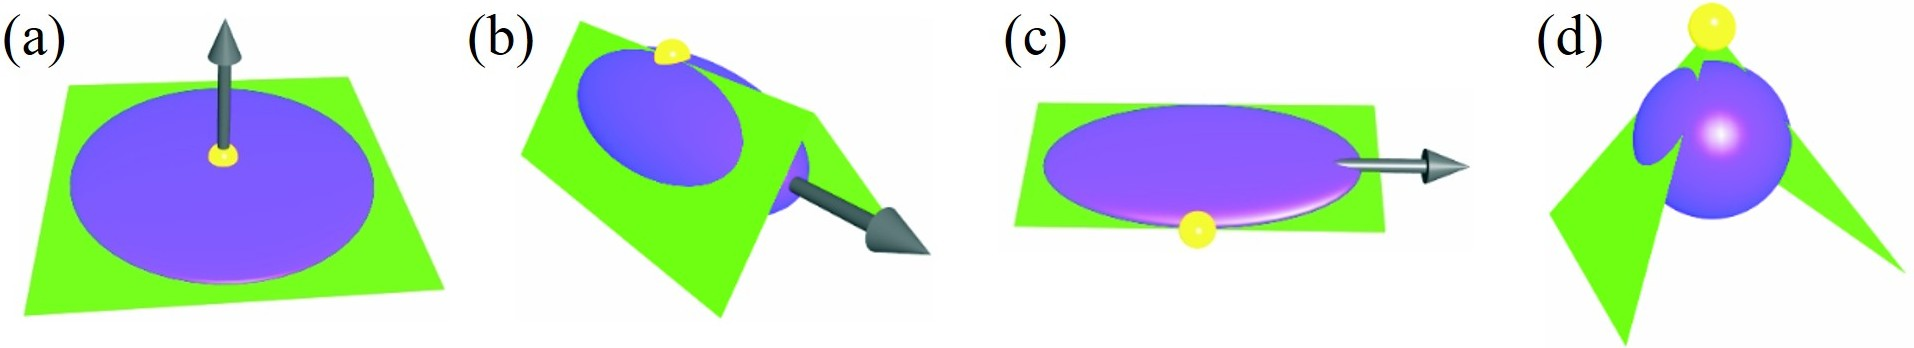
\includegraphics[width=0.85\textwidth]{Others/gumhold_feature_2001.jpg}
    \bicaption{不同几何特征点的邻域形状~\cite{gumhold_feature_2001}：(a) 平面点；(b) 折边点；(c) 边界点；(d) 角点。}{Neighborhood shapes of different geometric feature points~\cite{gumhold_feature_2001}: (a) Face point; (b) Ridge point; (c) Boundary point; (d) Corner point.}
    \label{fig:gumhold_feature_2001}
\end{figure}

在 PCA 方法的基础上，Xia等人~\cite{xia_fast_2017} 进一步引入了基于局部协方差矩阵的特征值比率的边缘检测算法，通过分析特征值之间的相对关系，实现几何特征的检测。Pauly等人~\cite{pauly_multiscale_2003} 和 Bazazian等人~\cite{bazazian_fast_2015} 则提出了多尺度分析框架，通过综合不同邻域尺度下的几何响应值来增强特征检测的鲁棒性。多尺度分析能够在一定程度上缓解单一尺度选择带来的问题，但仍然依赖于人工设定的阈值，且在处理具有复杂几何结构的物体时，特征点的界定仍然模糊不清。

Nguyen等人~\cite{nguyen_edge_2018} 基于曲率进行边缘特征提取并分为三个阶段：先利用曲率估计并配合阈值策略定位可能的边缘点；再通过迭代非极大值抑制对高曲率响应的宽带区域进行压缩与精炼，以获得更准确、稀疏的边缘点集合；最后基于距离阈值判定点与点之间的邻接关系，将相邻点逐步连接形成连续的特征线或边缘，从而实现稳定的线状特征恢复。王丽辉等人~\cite{WangLiHui_san_2011} 则结合曲率和法线信息进行邻域分析，并通过八叉树结构计算模型数据点密度，利用密度信息辅助边缘点的提取和连接，提升了边缘检测的准确性和连续性。

基于图的方法可以通过结合全局上下文信息进一步增强特征提取。例如，Demarsin等人~\cite{demarsin_detection_2007} 针对曲线的检测开展相关工作。其先基于点云法线信息，通过一阶分割获得候选特征点，并将其组织为图结构以恢复锐特征线；随后构建最小生成树以形成初始线结构，并通过后续的重连接过程将断裂的线段闭合，从而获得闭合特征线。此外，Che等人~\cite{che_multiscan_2018} 采样了一种无需通用法向估计的方法：首先设计了新的特征提取策略 NORmal VAriation ANAlysis（Norvana），能够剔除部分噪声点并提取边缘点；随后采用区域生长，将同一平滑曲面上的点聚合得到分割结果。图~\ref{fig:che_multiscan_2018} 展示了Norvana的结构。
\begin{figure}[htbp]
    \centering
    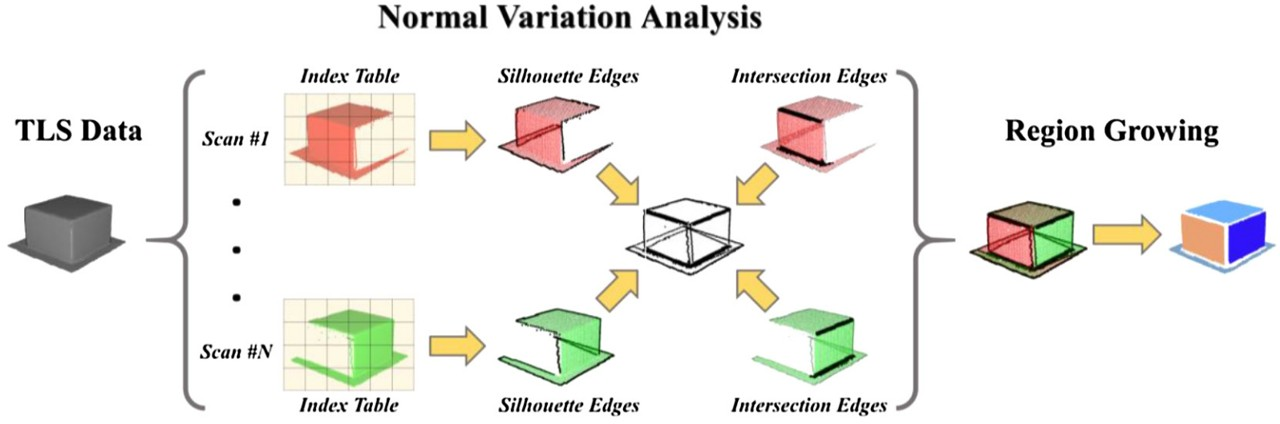
\includegraphics[width=0.85\textwidth]{Others/che_multiscan_2018.jpg}
    \bicaption{基于法向量分析的边缘检测方法Norvana~\cite{che_multiscan_2018}。}{Norvana: Normal Variation Analysis-based edge detection method~\cite{che_multiscan_2018}.}
    \label{fig:che_multiscan_2018}
\end{figure}

基于表面重建的方法，如利用移动最小二乘法（Moving Least Squares, MLS）~\cite{daniels_robust_2007}，可以通过利用局部近似来改善尖锐特征的检测。该方法首先在局部邻域内拟合一个高阶多项式曲面，然后分析数据点到拟合曲面的残差分布。特征点通常表现为拟合残差较大的区域，或者拟合曲面曲率极大的位置。这类方法的优势在于能够提供亚像素级别的特征定位精度，但高阶曲面拟合的计算开销较大，且在特征交汇复杂的角点区域容易产生伪影。Zhang等人~\cite{zhang_multinormal_2019} 提出了 VAM，利用成对一致性投票机制进行法向量估计，在尖锐边缘或角点处允许存在多个法向量假设，并通过邻域内的一致性投票来筛选出最能代表几何结构的法向量组合，从而有效地在重建过程中保留尖锐特征。

Lin等人~\cite{lin_line_2015} 则利用多视图投影点云的方法进行边缘检测。如图~\ref{fig:lin_line_2015} ，其将三维点云进行多视图投影，再基于二维图像的线段检测算法（LSD）进行边缘提取，最后将检测到的线段重新映射回三维空间。并利用半平面线段分割结构（Line-Segment-Half-Planes, LSHP）进行进一步的匹配，得到完整的三维线段特征。该方法通过引入多视图投影的策略，成功地将二维图像处理技术应用于三维点云的边缘检测中。
\begin{figure}[htbp]
    \centering
    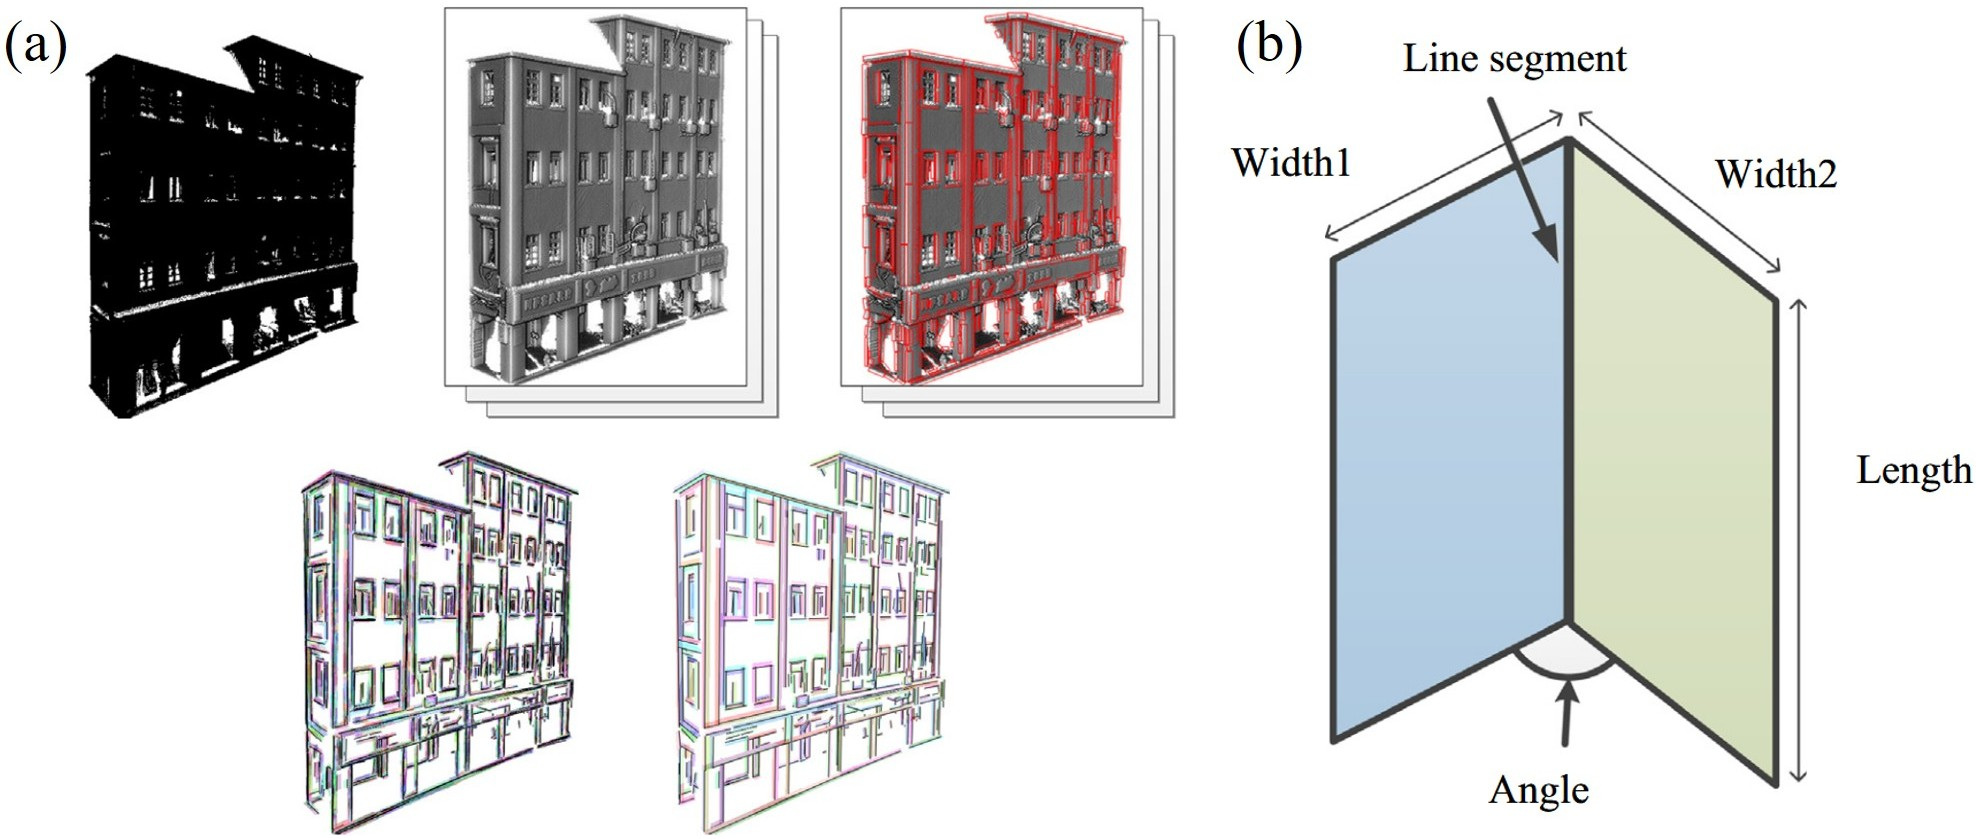
\includegraphics[width=0.85\textwidth]{Others/lin_line_2015.jpg}
    \bicaption{基于多视图投影的三维点云边缘检测流程~\cite{lin_line_2015}：(a) 各阶段检测结果；(b) LSHP结构示意图。}{Multi-view projection-based 3D point cloud edge detection pipeline~\cite{lin_line_2015}: (a) The detection results of each stage; (b) Schematic of the LSHP structure.}
    \label{fig:lin_line_2015}
\end{figure}

在角点检测方面，针对仅提取边缘不足以描述完整几何特征的问题，Ahmed等人~\cite{ahmed_edge_2018} 采用了两步提取过程：首先基于邻域的空间分析区分出面点和非面点，然后利用聚类的方法在非面点中识别角点。此外，Schmidt等人~\cite{schmidt_detection_2023} 提出使用 RANSAC 算法从点云中提取直线或平面，并在它们的交点处检测角点。这些方法尝试通过几何基元的组合关系来定位角点，但在复杂噪声环境下仍面临挑战。

综上所述，虽然以几何描述符、表面重建及图优化为代表的传统解析方法为点云特征提取奠定了理论基础，并在规则模型的边缘检测中表现出一定有效性，但其局限性亦十分显著。首先，这类方法本质上依赖于人工设计的几何规则与先验假设，对噪声极其敏感，且高度依赖如邻域尺度、曲率阈值等参数的精细调节，难以在物体形状多变、数据质量参差的现实场景中实现自适应的稳健检测。其次，基于平滑拟合的策略往往导致尖锐特征被过度平滑，造成定位精度损失。最为关键的是，角点检测在此类方法中常被边缘化，多作为边缘提取后的二次处理步骤或依赖于理想化的平面相交假设，这种两阶段策略不仅计算冗余，且在处理复杂拓扑结构的角点时极易因特征模糊而产生误检或漏检。

\subsubsection{基于数据驱动的方法}
近年来，随着深度学习在三维视觉领域的突破，基于数据驱动的几何特征检测方法逐渐成为主流。这类方法通常将特征提取任务建模为分类或回归问题，将点云中的每个点标记为属于特定的几何类别或找出拟合的几何参数。相较于传统方法，数据驱动模型不再依赖人工设定的复杂阈值，而是通过神经网络自动学习从局部几何结构到特征类别的映射关系，展现出更强的鲁棒性和泛化能力。

点云数据存在无序、稀疏且高维的特点，传统卷积神经网络难以直接应用于点云数据的处理。随着 PointNet~\cite{charles_pointnet_2017a} 及其改进版本 PointNet++~\cite{qi_pointnet_2017} 的提出，直接处理点云数据的深度学习方法得以实现。基于此架构，研究者们设计了多种网络结构来针对边缘和角点的检测进行优化。例如，Wang 等人提出的 PIE-Net~\cite{wang_pienet_2020} 基于 PointNet++ 设计了两个相同的网络分别用于边缘和角点的检测。其实现了点云边缘和角点检测的端到端检测。然而，PIE-Net 的分离提取设计效率较低，需要对角点检测结果进行后处理，且网络对输入点数有严格限制，难以适应大规模点云场景。

\begin{figure}[htbp]
    \centering
    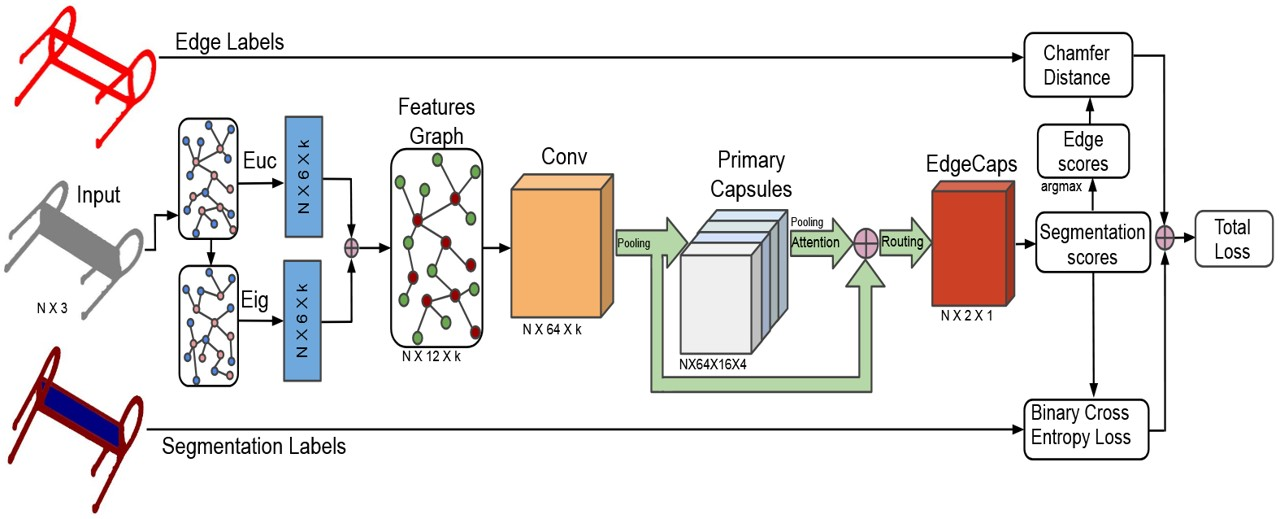
\includegraphics[width=0.95\textwidth]{Others/bazazian_edcnet_2021.jpg}
    \bicaption{基于胶囊网络的边缘检测方法 EDC-Net~\cite{bazazian_edcnet_2021}。}{EDC-Net: Capsule network-based method for edge detection~\cite{bazazian_edcnet_2021}.}
    \label{fig:bazazian_edcnet_2021}
\end{figure}
针对特征空间层级关系的建模，Bazazian 等人提出的 EDC-Net~\cite{bazazian_edcnet_2021} 引入了胶囊网络（Capsule Network），如图~\ref{fig:bazazian_edcnet_2021} 所示。该方法首先将局部邻域编码为几何描述符，利用胶囊层独特的动态路由机制来捕捉特征的空间分布结构，从而将点稳健地分类为非边缘或锐利边缘，减少了对人工参数的依赖。此外，针对输入形式的不同，Guerrero 等人的 PCPNet~\cite{guerrero_pcpnet_2018} 专注于局部几何属性的估计，它以多尺度的点云局部图块（Patches）作为输入，通过共享权重的 MLP 学习局部形状特征，不仅能估计法向量和曲率，也能用于特征点的分类。Jiao 等人的 MSL-Net~\cite{jiao_mslnet_2024} 则提出了一种轻量级的多尺度局域网络，通过在不同半径下聚合局部邻域信息增强特征表达，旨在解决大规模点云场景下边缘提取的实时性问题。

为了更有效地利用局部几何信息，Himeur 等人提出的 PCEDNet~\cite{himeur_pcednet_2022} 和 Bode 等人提出的 BoundED~\cite{bode_bounded_2023} 采用了基于多尺度局部特征描述符的策略。这类方法首先计算点云的多尺度几何属性（如曲率、法向量分布等），然后将这些描述符输入 MLP 进行特征融合与分类。研究表明，通过神经网络学习局部描述符的非线性组合，可以显著提升边缘检测的精度。然而，由于边缘和角点在局部邻域内的几何特征极具相似性，现有方法仍未运用于角点的检测，无法证明其有效性。

除了将被检测任务视为逐点分类问题，部分研究将其重构为回归问题或采用不同的数据表征。Yu 等人提出的 EC-Net~\cite{yu_ecnet_2018}不直接进行二分类，而是学习预测每个点到最近边缘的距离场（Distance Field）。通过回归距离值为零的等值线，EC-Net 能够以亚像素级的精度恢复出锐利的边缘曲线，尤其在处理倒角特征时表现优异。类似的，Matveev 等人的 DEFs~\cite{matveev_def_2022} 采用了一种隐式场回归的策略。该网络训练模型回归每个查询点到最近边缘曲线的距离以及特征点的坐标残差，随后通过后处理算法重建高精度的连续边缘线。

\begin{figure}[htbp]
    \centering
    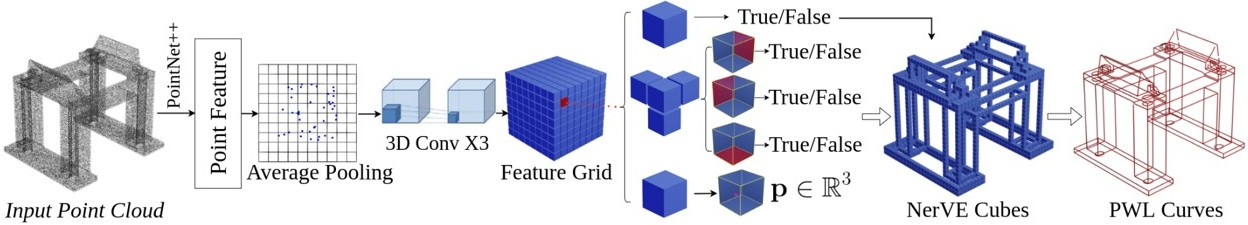
\includegraphics[width=1.0\textwidth]{Others/zhu_nerve_2023.jpg}
    \bicaption{基于体素网格的边缘检测方法 NerVE~\cite{zhu_nerve_2023}。}{NerVE: Voxel-based edge detection method~\cite{zhu_nerve_2023}.}
    \label{fig:zhu_nerve_2023}
\end{figure}
在数据表征方面，Zhu 等人提出的 NerVE~\cite{zhu_nerve_2023} （如图~\ref{fig:zhu_nerve_2023} 所示）针对无序点云难以进行常规卷积的问题，将点云转化为规则的体素（Voxel）网格。该方法利用稀疏三维卷积神经网络提取体素特征，并在体素内进一步进行节点分类，在保持结构化感知的同时实现了对尖锐几何特征的有效检测。Hu 等人的 JSENet~\cite{hu_jsenet_2020} 则将任务扩展为三维语义边缘检测，采用双流全卷积架构，一支流负责语义分割，另一支流专注边缘检测，通过特征交互模块融合两者的信息，从而在提取几何边缘的同时赋予其语义类别属性。这种方法的检测结果不仅具有几何准确性，还能提供丰富的语义信息，但其处理效率较低，在大规模点云场景下的适应性有待提升。

总体而言，目前的学习型方法主要集中在边缘特征提取上，且效果显著，但针对角点检测的研究相对匮乏。PCEDNet 和 BoundED 等方法证明了通过神经网络学习局部几何描述符在边缘检测上的有效性。基于此，本文延续并改进这一技术路线：针对角点和边缘难以区分的难点，本文对计算特征描述符进行针对性的设计，提出了能够有效辨识角点的新型几何特征，并采用基于 MLP 的层次化网络结构来学习这些特征，从而实现对面、边缘和角点三类特征的高精度同步检测。

\subsection{机器人抓取规划研究现状}
机器人抓取规划主要可以分为抓取构型（Grasp Configuration）规划和抓取质量评估两个方面。这两部分都包括基于分析和数据驱动的方法。
\subsubsection{抓取构型规划}
机器人抓取规划方法通常可分为基于模型（Model-based）和基于学习（Learning-based）的方法。基于模型的方法依赖于物体的几何信息和物理规则来生成抓取构型，这类方法进一步可分为两种主要策略：图元拟合（Primitive Fitting）和表面分割（Surface Segmentation）。

图元拟合策略使用基本的几何图元（如圆柱体、球体、方块等）来近似物体，从而简化抓取合成过程~\cite{goldfeder_grasp_2007}。Miller 等人提出了 GraspIt! 仿真器~\cite{miller_automatic_2003,miller_graspit_2021}，通过将复杂物体分解为一组简单的几何原语来快速生成抓取假设。Chen 等人~\cite{chen_category_2022} 利用词嵌入（Word Embeddings）来量化已知模型类别与真实物体之间的语义相似度，从而实现新物体与数据库模型的匹配。虽然图元近似降低了计算复杂度，但它往往丢失了物体的局部细节几何信息，导致生成的抓取难以适应具有丰富几何特征的复杂物体。
\begin{figure}[htbp]
    \centering
    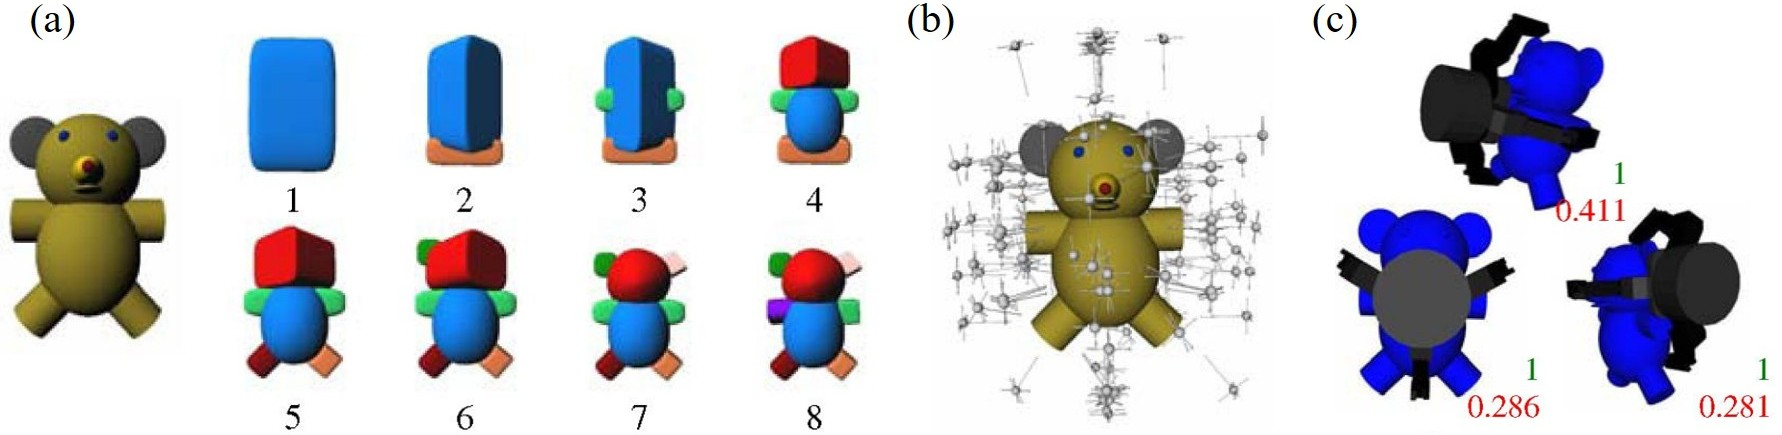
\includegraphics[width=0.95\textwidth]{Others/goldfeder_grasp_2007.jpg}
    \bicaption{基于图元拟合的抓取规划方法~\cite{goldfeder_grasp_2007}：(a) 图元拟合过程；(b) 抓取构型生成；(c) 抓取质量评估。}{Grasp planning method based on primitive fitting~\cite{goldfeder_grasp_2007}: (a) Primitive fitting process; (b) Grasp configuration generation; (c) Grasp evaluation.}
    \label{fig:goldfeder_grasp_2007}
\end{figure}

表面分割策略则致力于识别有意义的表面区域以指导抓取生成。Harada 等人~\cite{harada_grasp_2011} 针对软指尖手爪，根据接触软度对三角网格进行聚类，规划出适应物体局部曲率的抓取。Wan 等人~\cite{wan_planning_2021} 引入了叠加分割（Superimposed Segmentation）技术，根据表面法向量将每个三角形分割为具有受控重叠和厚度的多个面片。然而，为了确保力封闭的稳定性，这类方法通常显式地剔除边缘和角点附近的区域，避免在曲率突变处建立接触~\cite{wan_planning_2021, miller_graspit_2021}。这种“面接触优先”的策略虽然提高了抓取的保守稳定性，却极大限制了抓取构型在物体表面的分布，导致灵活性不足。
\begin{figure}[htbp]
    \centering
    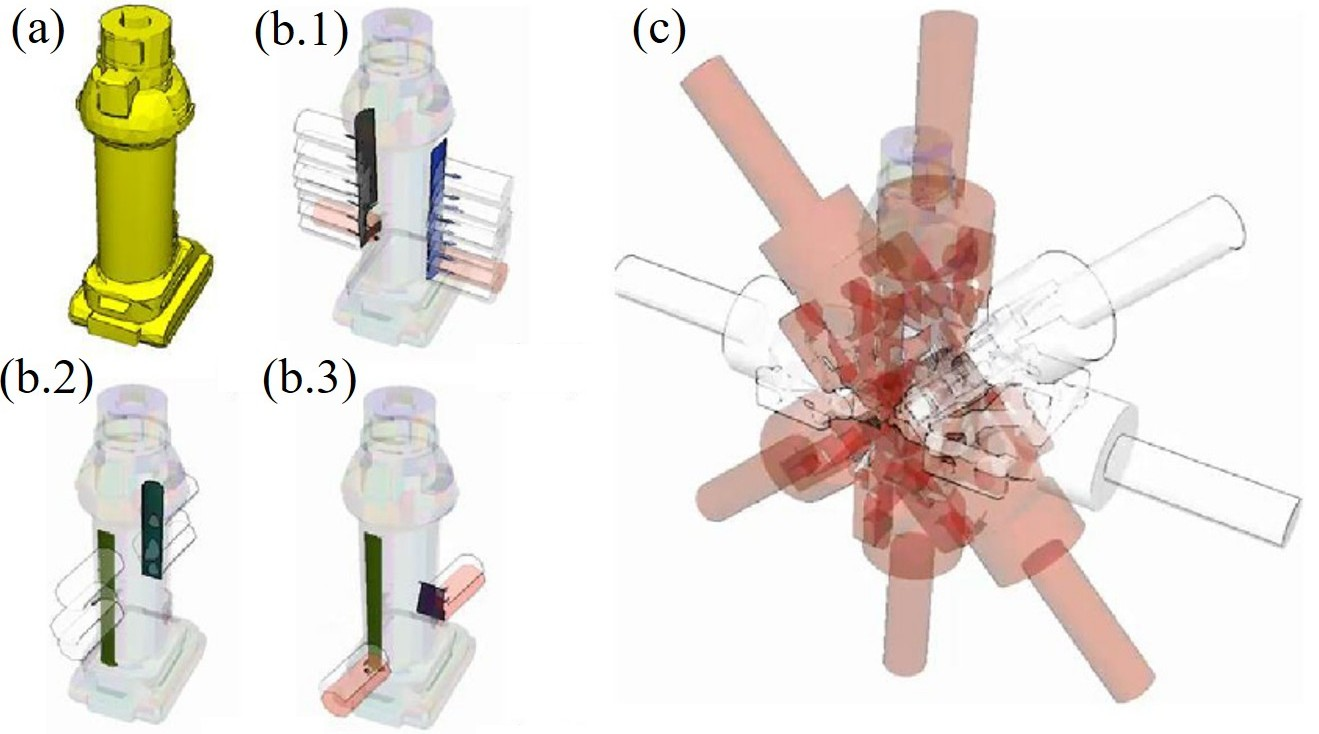
\includegraphics[width=0.6\textwidth]{Others/wan_planning_2021.jpg}
    \bicaption{基于表面分割的抓取规划方法~\cite{wan_planning_2021}：(a)物体模型；(b.1-3)表面分割结果；(c)抓取构型生成。}{Grasp planning method based on surface segmentation~\cite{wan_planning_2021}: (a) Object model; (b.1-3) Surface segmentation results; (c) Grasp configuration generation.}
    \label{fig:wan_planning_2021}
\end{figure}

另一方面，基于学习的方法利用神经网络和数据驱动技术来增强抓取的泛化能力。Mahler 等人提出的 Dex-Net~\cite{mahler_dexnet_2017,mahler_learning_2019} 系列构建了大规模的合成抓取数据集，训练卷积神经网络（GQ-CNN）直接从深度图像中预测平面抓取的成功率。Mousavian 等人~\cite{mousavian_graspnet_2019} 则提出了 6-DOF GraspNet，通过基于变分自编码器（VAE）的框架生成多样化的6自由度抓取构型。该方法利用抓取评价或精炼网络对候选进行评分并迭代优化，以提高抓取的稳定性与可执行性；最终结合碰撞检测等几何约束过滤不可行抓取，实现对复杂物体的多样化6D抓取构型生成。
\begin{figure}[htbp]
    \centering
    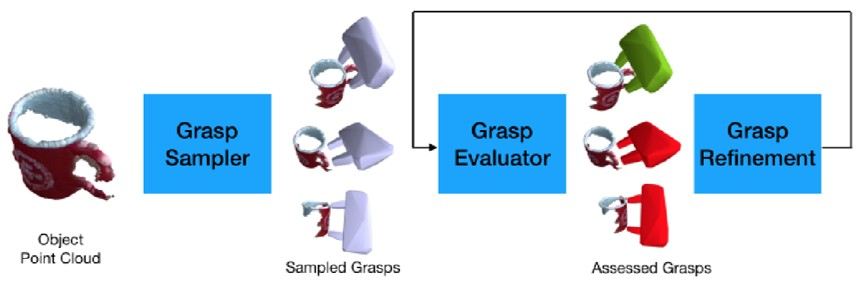
\includegraphics[width=0.9\textwidth]{Others/mousavian_graspnet_2019.jpg}
    \bicaption{基于变分自编码器的6-DOF抓取生成方法~\cite{mousavian_graspnet_2019}。}{6-DOF grasp generation method based on variational autoencoder~\cite{mousavian_graspnet_2019}.}
    \label{fig:mousavian_graspnet_2019}
\end{figure}

尽管这些方法在未见过物体上表现出色，但其训练数据通常是基于传统解析指标（如 GraspIt! 中的能量函数）生成的~\cite{fang_graspnet1billion_2020}。因此，数据驱动模型倾向于继承“排斥边缘”的偏见，将边缘和角点视为噪声或不稳定区域，从而难以生成涉及这些尖锐特征的多样化抓取~\cite{mahler_learning_2019, cao_efficient_2023}。
本文提出的方法打破了这一局限，引入软接触模型，将潜在的稳定接触扩展到边缘和角点。通过开发包含边缘和角点接触的抓取规划算法，旨在显著增加抓取分布的覆盖率和灵活性。

\subsubsection{抓取质量评估}
为了评估抓取候选的可行性和质量，研究者提出了多种抓取评价标准。最常用的解析指标是抓取稳定性，通常通过力封闭（Force Closure）或形封闭（Form Closure）条件进行评估~\cite{bicchi_robotic_2000}。解析方法通过评估旋量空间覆盖率（Wrench Space Coverage）、抗扭矩能力或最小力需求来确定抓取的可靠性。Ferrari 和 Canny~\cite{ferrari_planning_1992} 提出了经典的 $\epsilon$ 指标，通过计算抓取矩阵在旋量空间中张成的最大球半径（$L_2$ 范数）或最大多胞体体积（$L_1$ / $L_\infty$ 范数）来量化抓取抵抗外部扰动的能力。然而，这些解析指标通常假设刚性接触，对于边缘和角点这类理论上接触面积为零的区域，往往给出极低的稳定性评分。

相比之下，数据驱动方法通常训练模型直接从视觉或几何输入预测抓取质量评分。Ten Pas 等人提出的 GPD（Grasp Pose Detection）算法~\cite{tenpas_grasp_2017} 则直接在三维点云中采样候选抓取，并对物体点云进行投影，利用CNN网络评估其抓取质量。Liang 等人则对 GPD 的抓取质量评估网络进行了改进，提出了基于 PointNet++ 的 PointNetGPD~\cite{liang_pointnetgpd_2019}，通过引入多尺度特征融合和注意力机制来提升评估的准确性和鲁棒性，并且无需对点云进行投影。
\begin{figure}[htbp]
    \centering
    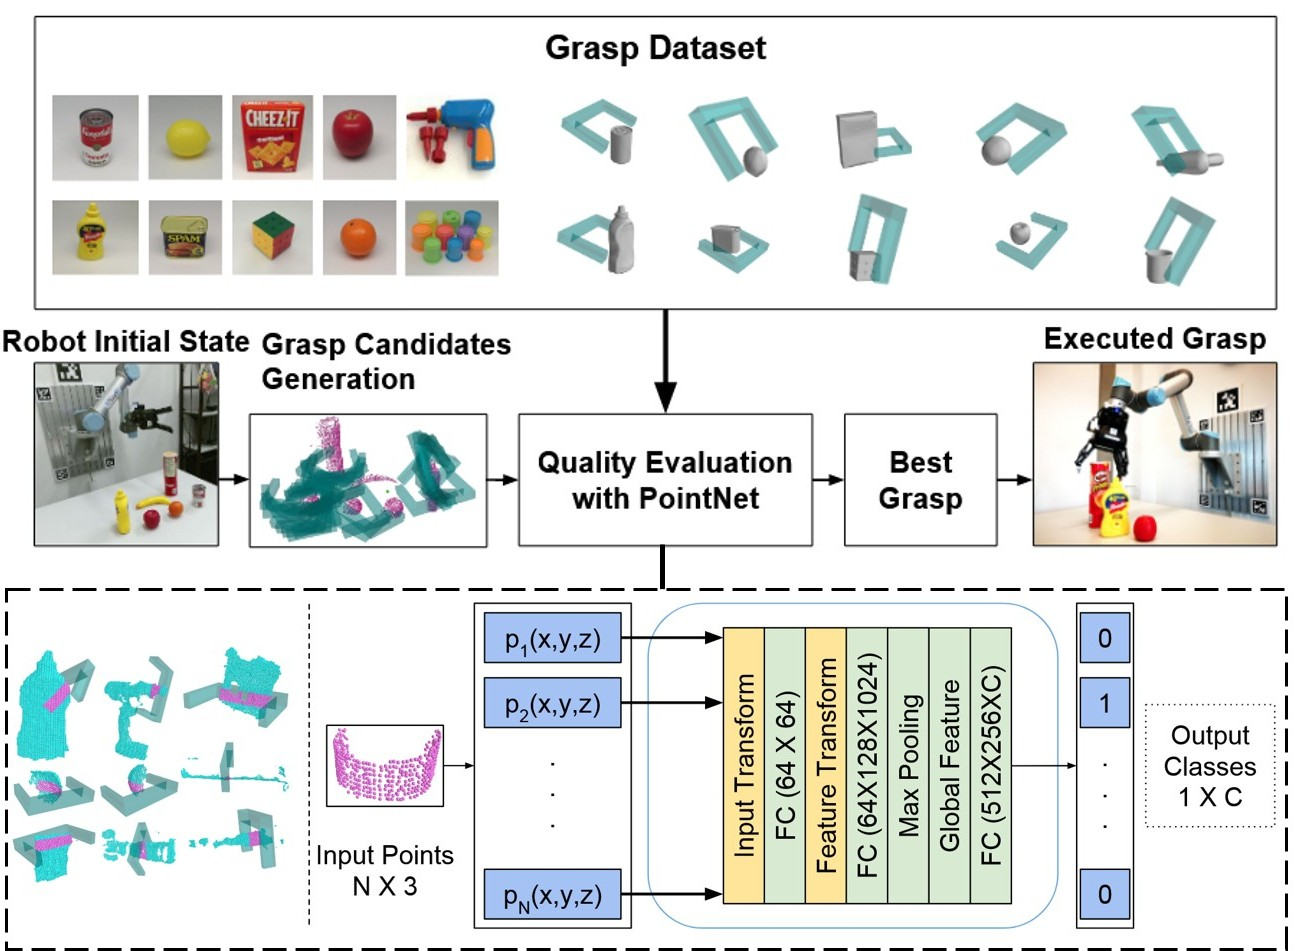
\includegraphics[width=0.85\textwidth]{Others/liang_pointnetgpd_2019.jpg}
    \bicaption{基于深度学习的抓取质量评估方法 PointNetGPD~\cite{liang_pointnetgpd_2019}。}{PointNetGPD: Grasp Pose Detection method based on deep learning~\cite{liang_pointnetgpd_2019}.}
    \label{fig:liang_pointnetgpd_2019}
\end{figure}

近期，Yu 等人~\cite{yu_mtgrasp_2025} 和 Cao 等人~\cite{cao_efficient_2023} 引入了更先进的深度网络架构来捕捉抓取区域的全局上下文信息，进一步提升了评估的准确性。虽然这些学习模型可能缺乏如力封闭等形式化保证，但它们在非结构化和实时环境中表现出了卓越的适应性。此外，一些混合方法结合了解析指标与数据驱动模型，以增强泛化能力和鲁棒性~\cite{kopicki_learning_2014}。

值得注意的是，现有的大多数评价指标主要关注单个抓取构型的成功率或稳定性，而缺乏对规划器生成的抓取解集在物体表面空间分布情况的量化评估。针对这一问题，本文引入了一种基于统计熵的指标，用于量化抓取构型的分布均匀性，并作为抓取灵活性的代理指标。该指标能够对不同规划器在抓取灵活性方面进行定量且直观的比较，而不受其选择接触区域优先级的差异影响。

\section{本文主要研究内容}
\label{sec:contribution}

针对物体几何特征检测中存在的角点识别困难、检测精度不足的问题，以及机器人抓取规划中因过分依赖面接触而导致的抓取灵活性受限问题，本文开展了系统性的研究工作。本文的核心目标是建立一套从高精度几何感知到灵活多模式抓取规划的完整技术方案。本文的主要研究内容包括以下两个方面：

第一，本文提出了一种基于多尺度局部特征融合的点云边缘与角点检测流程框架（NECDNet）。针对现有方法在角点检测上的缺失，该研究设计了一套包含曲率、投影距离、法向分布等六个维度的解析特征描述符，专门用于捕捉稀疏且模糊的角点信号。通过构建多尺度邻域特征矩阵作为输入，并设计基于多层感知机（Multi Layer Perceptron, MLP）的层次化分类网络，该方法实现了对点云中面、边缘、角点三类特征的高精度端到端识别。如图~\ref{fig:necdnet_result} 所示，较其余方法，该网络不仅保持了边缘检测的高性能，更显著提升了角点检测的准确率。

\begin{figure}[htbp]
    \centering
    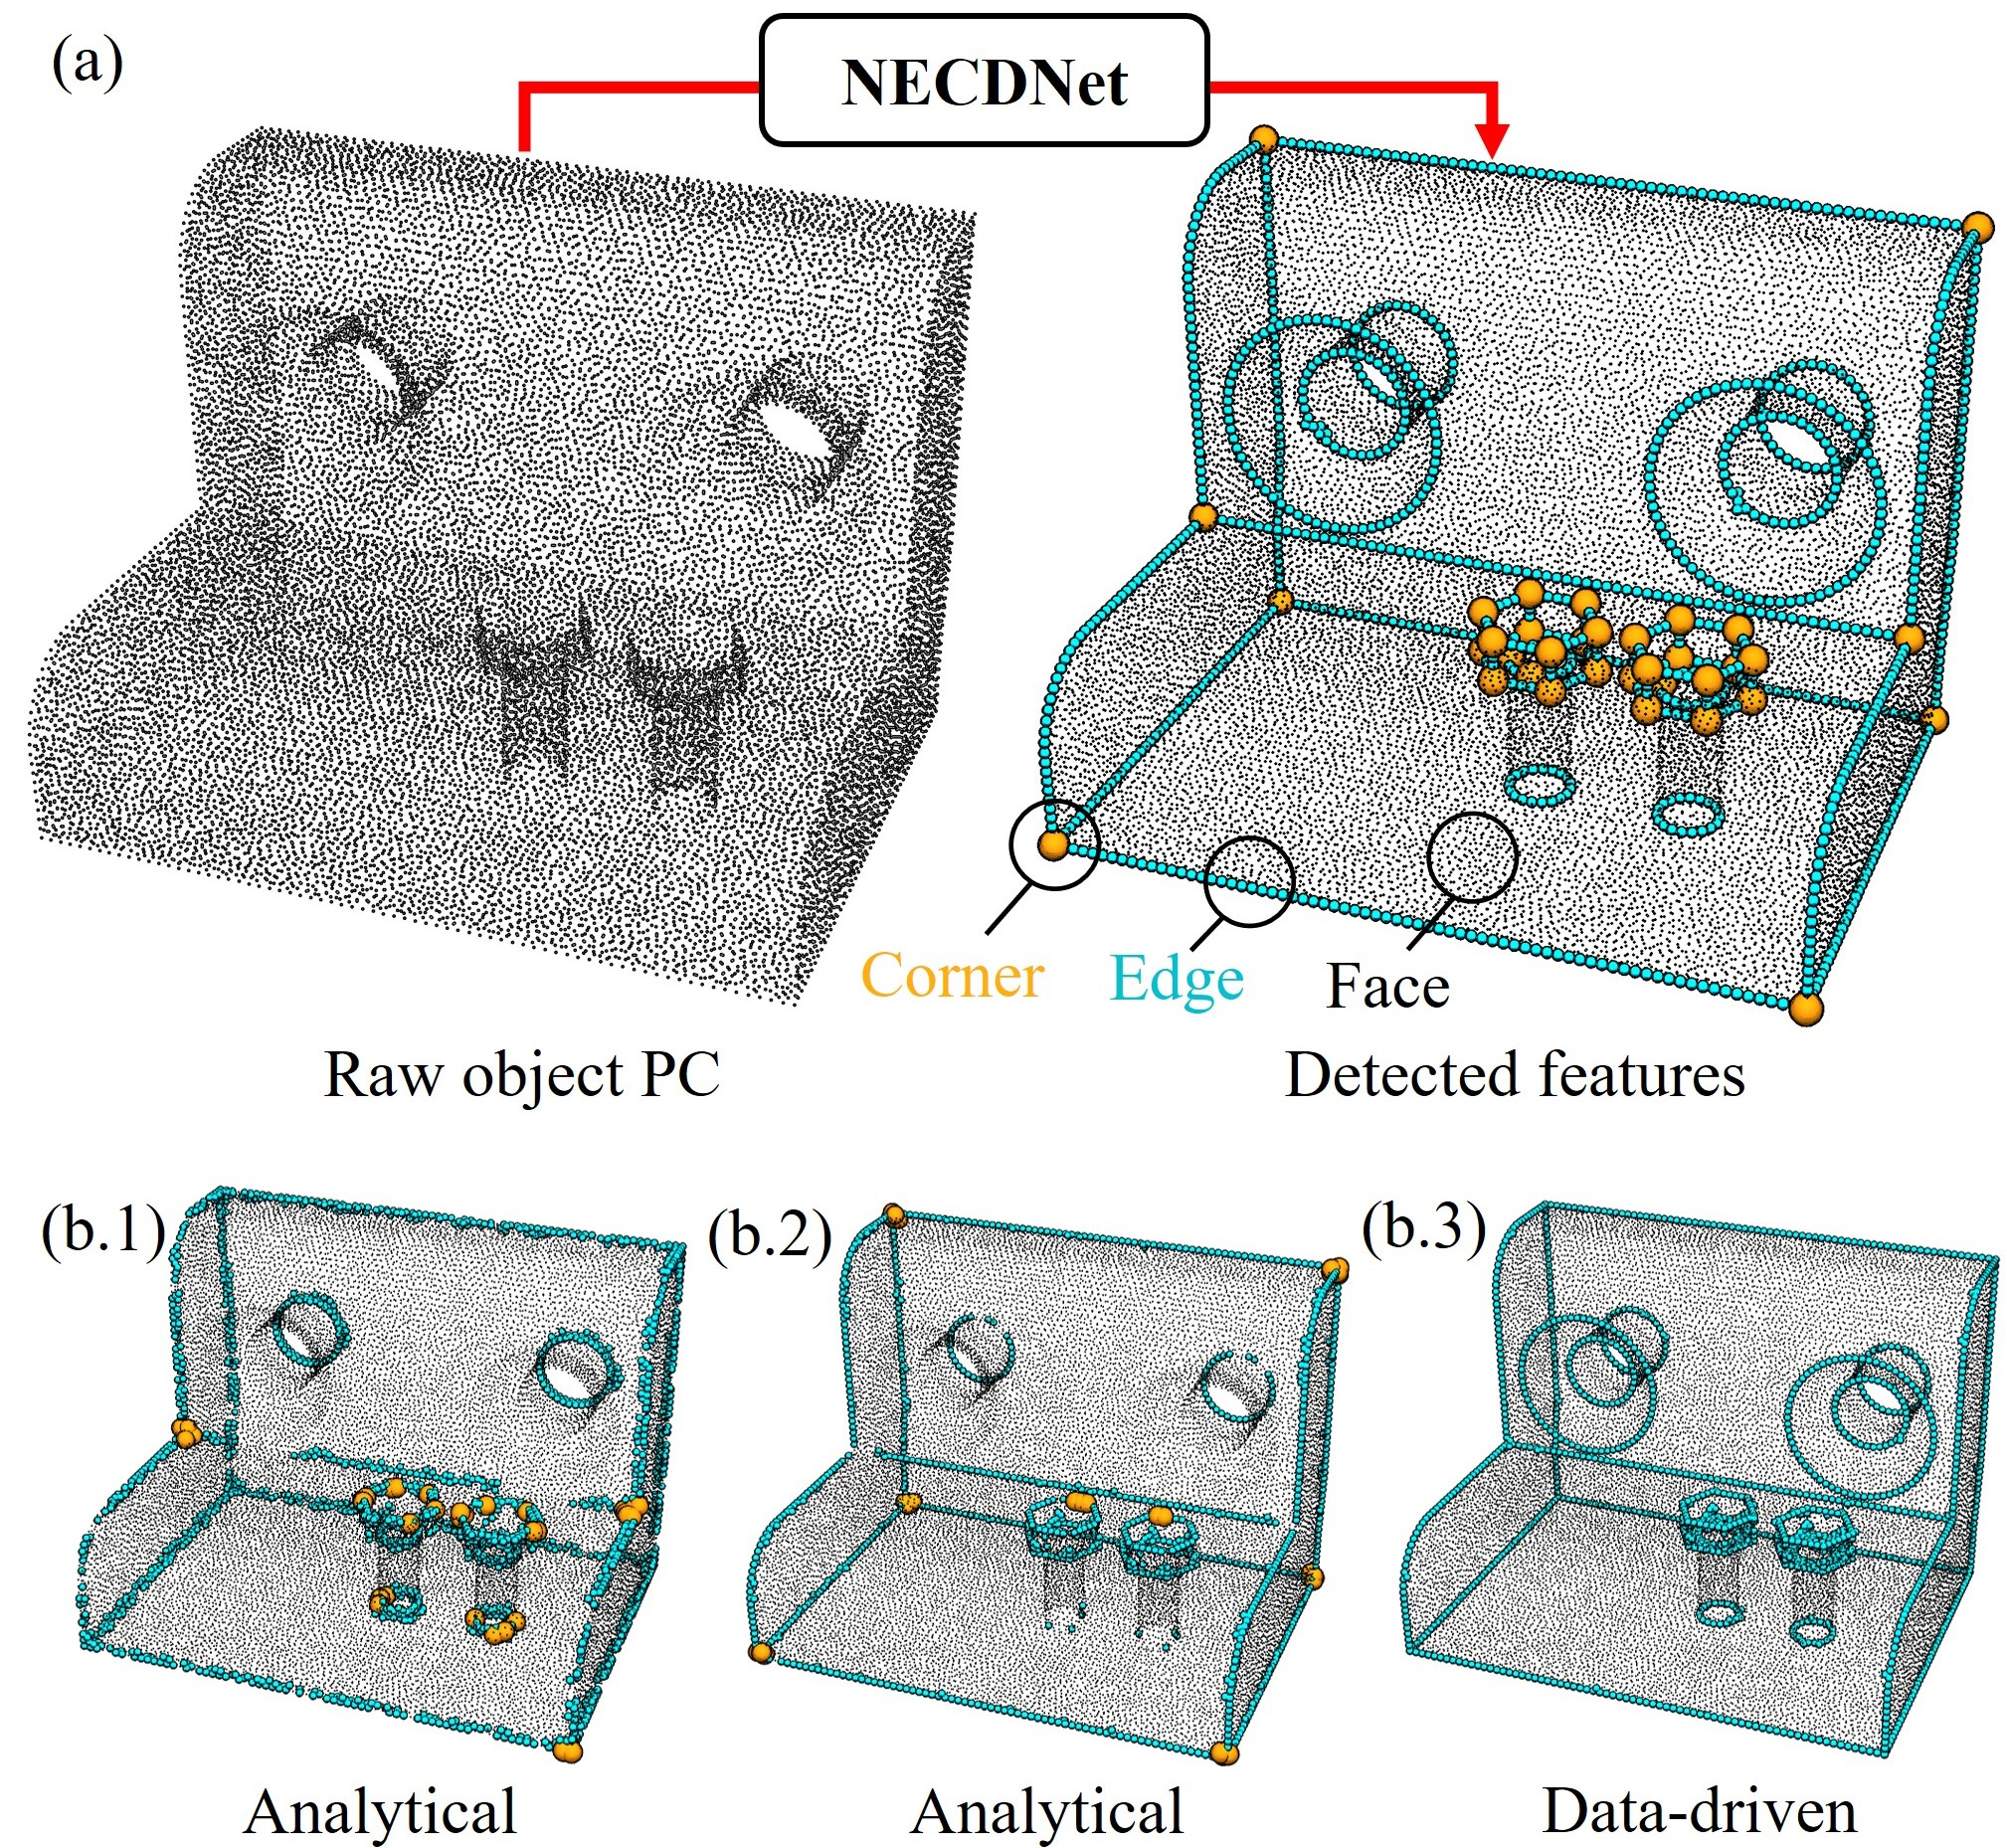
\includegraphics[width=1.0\textwidth]{NECDNet/teaser.jpg}
    \bicaption{不同几何特征检测方法结果对比：(a) NECDNet；(b.1-3) CA~\cite{gumhold_feature_2001}, TECD~\cite{ahmed_edge_2018}, PCEDNet~\cite{himeur_pcednet_2022}。}{Comparison of geometric feature detection results: (a) NECDNet; (b.1-3) CA~\cite{gumhold_feature_2001}, TECD~\cite{ahmed_edge_2018}, PCEDNet~\cite{himeur_pcednet_2022}.}
    \label{fig:necdnet_result}
\end{figure}

其中，为了解决深度学习方法在几何特征检测领域面临的训练数据匮乏问题，本文构建了 ABC-Corner 基准数据集。该数据集从大规模 CAD 模型库 ABC 数据集中精选了 1000 个具有丰富几何细节的代表性模型。通过结合基于几何规则的自动初筛算法与人工精细交互修正的标注流程，生成了包含面、边缘、角点三类高精度标签的点云数据。该数据集填补了领域内缺乏专门针对角点检测的大规模公开数据集的空白，为后续的数据驱动算法研究提供了可靠的基准。

第二，本文提出了一种考虑边缘和角点接触的六自由度机器人抓取规划算法。该算法突破了传统面接触优先的规划范式，将边缘和角点纳入可行的接触候选区域。算法利用提取的几何特征进行类别感知的均衡采样，并针对面、边、角三种不同特征分别设计了圆柱形、扇形和圆锥形接触检测器，以高效搜索潜在的对指抓取配对。通过引入基于离散化的软指接触模型，实现了对边缘和角点接触稳定性的有效评估。此外，本文还首次引入了抓取分布统计指标来量化评估抓取规划的灵活性。如图~\ref{fig:fbgrasp_result} 展示了该算法生成的抓取构型，实验结果证明，该方法在正四面体、非对称曲面等复杂物体上实现了极高的抓取成功率和空间覆盖率。

\begin{figure}[htbp]
    \centering
    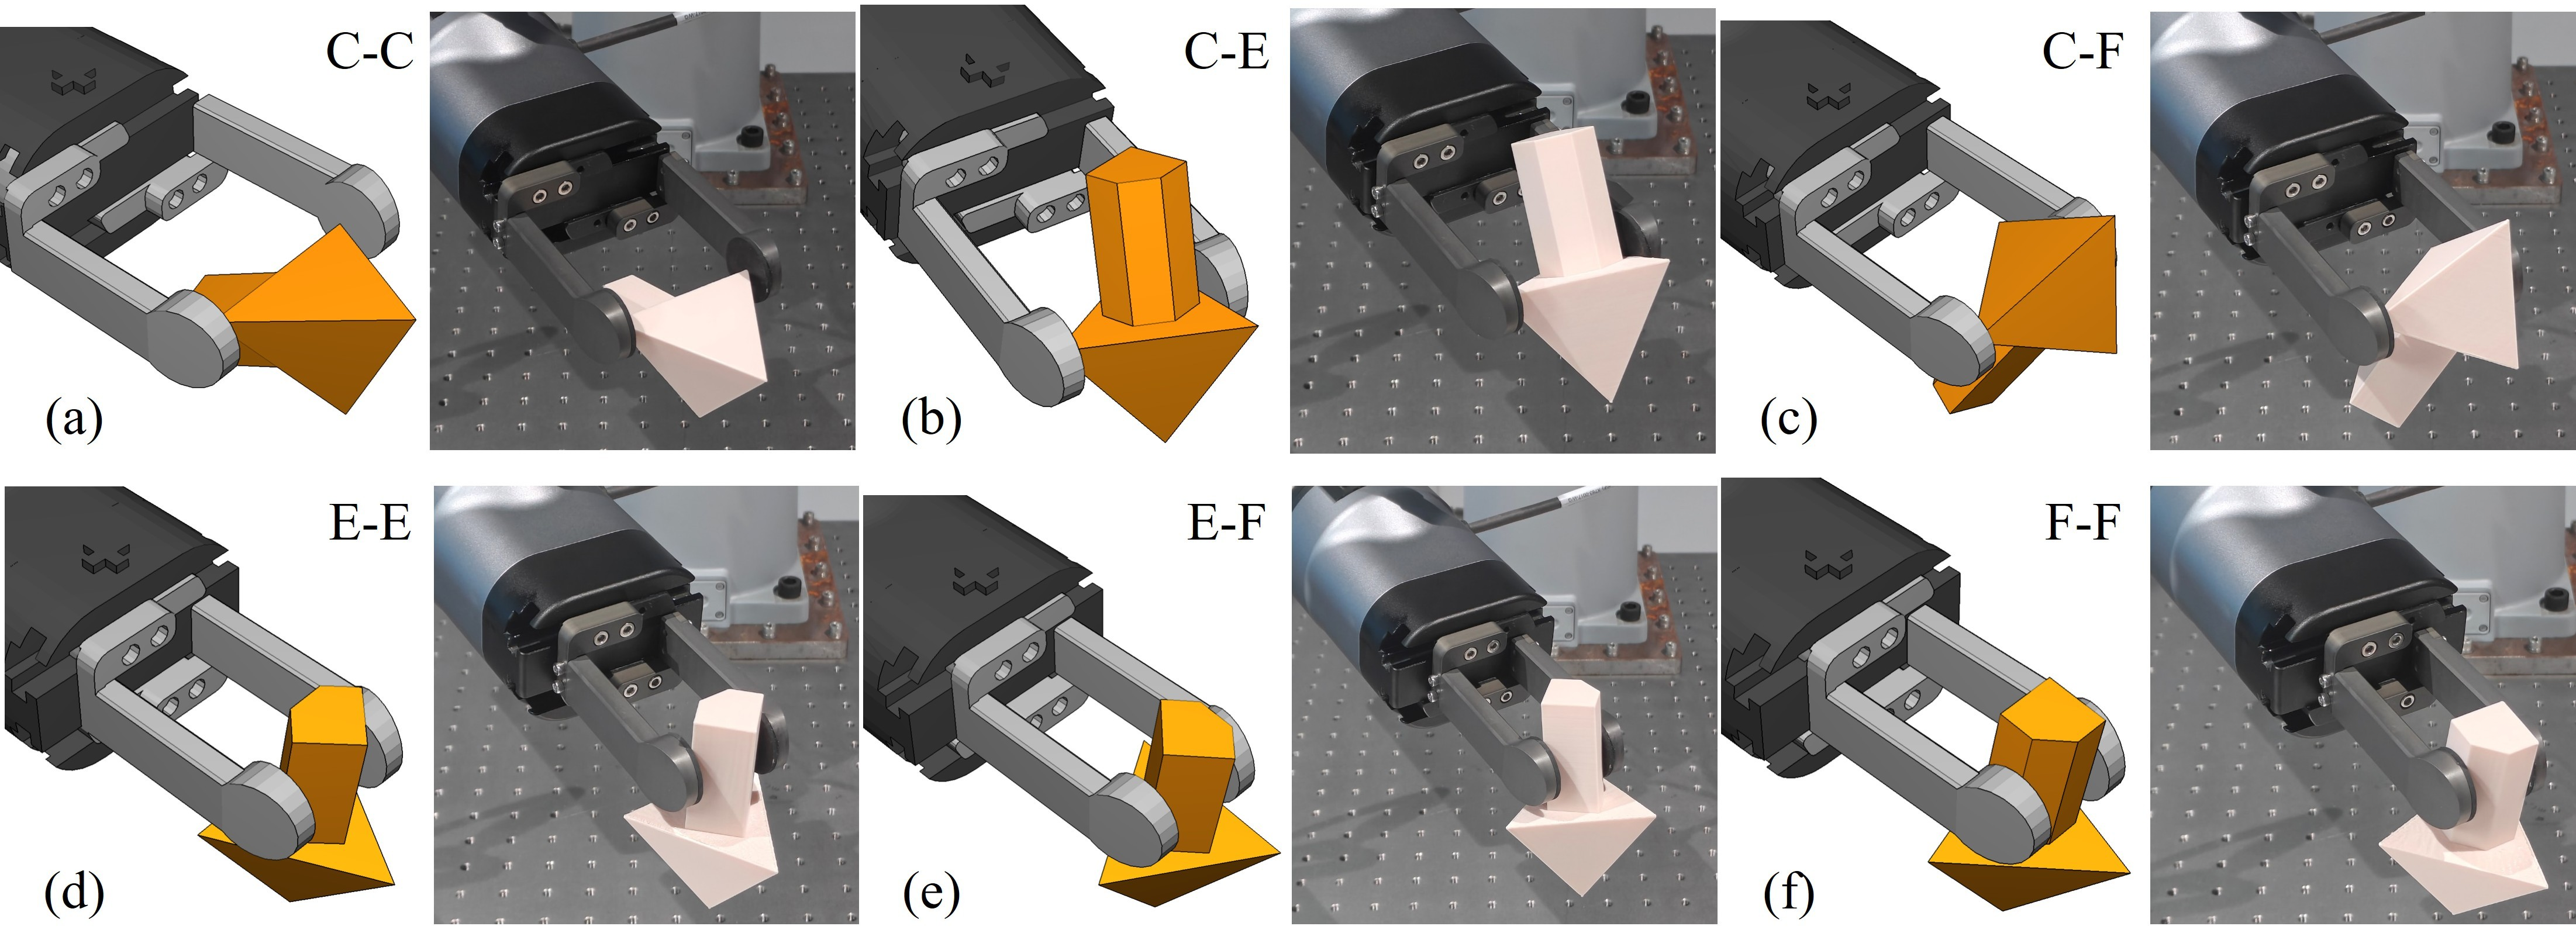
\includegraphics[width=1.0\textwidth]{FBGrasp/teaser.jpg}
    \bicaption{基于物体几何特征的抓取规划结果展示：(a-f) 针对三种几何特征实现的六种抓取构型，依次为：角-角，角-边，角-面，边-边，边-面，面-面。}{Grasp planning results based on object geometric features: (a-f) Six grasp configurations for three geometric features, including C-C, C-E, C-F, E-E, E-F, and F-F.}
    \label{fig:fbgrasp_result}
\end{figure}

综上所述，本文的主要创新点可以归纳为以下三个方面：

（1）提出了一种融合显式几何描述符与数据驱动的基于物体点云的几何特征检测网络（NECDNet）。 通过引入多尺度显式几何特征描述符，解决了纯数据驱动方法在稀疏角点检测上的特征模糊问题，实现了对面、边缘和角点的高精度同步检测。

（2）构建了包含高精度角点标注的大规模点云几何特征数据集（ABC-Corner）。针对现有数据集缺乏角点标注的问题，建立了一套半自动化的精细标注流程，为几何特征检测领域提供了高质量的数据基准。

（3）提出了一种基于软接触模型并融合边缘与角点接触的抓取规划算法。该算法突破了传统面接触优先假设，针对不同几何特征设计了专门的抓取构型检测策略，并引入抓取分布统计指标以量化评估抓取灵活性，同时采用软接触模型进行抓取稳定性评估，从而显著提升了机器人在复杂物体抓取任务中的灵活性和空间覆盖率。

\section{论文组织结构}
\label{sec:structure}

本文共分为六章，各章节的具体内容安排如下：

第一章为绪论，主要阐明点云几何特征检测与机器人抓取规划的研究背景和工程意义，系统梳理国内外相关研究进展，分析现有方法在角点检测精度与抓取灵活性方面的不足，并据此明确本文的研究目标、技术路线与主要创新点。

第二章围绕点云几何特征检测方法展开，重点介绍 NECDNet 的整体框架与实现过程，包括多尺度 $k$ 近邻邻域构建、六维显式几何描述符设计以及基于多层感知机的层次化分类结构。

第三章在上述方法基础上开展实验评估，首先给出 ABC-Corner 数据集的构建流程，为后续实验提供数据基础。之后通过与主流方法的定性和定量对比验证 NECDNet 在边缘与角点检测任务中的性能优势，并结合消融实验进一步分析特征维度、网络模块及法向量估计精度对结果的影响。

第四章进一步面向机器人抓取规划问题，提出一种考虑边缘与角点接触的六自由度抓取规划方法，系统介绍类别感知采样、面/边/角接触检测器设计、接触对构建与软接触稳定性评估等关键环节，形成从几何特征到抓取构型生成的完整流程。

第五章对所提抓取规划方法进行实验验证，分别从仿真与真实物理实验两个层面评估其性能，并通过抓取分布统计指标、抓取成功率指标与对比方法进行综合分析，验证方法在复杂几何物体上的有效性与实用性。最后分析了算法计算效率。

第六章对全文工作进行总结，归纳本文在物体几何特征检测与机器人抓取规划两方面的主要贡献，客观讨论当前方法的局限，并结合机器人操作场景的发展需求给出后续研究方向与改进思路。












% !Mode:: "TeX:UTF-8"
\chapter{基于多尺度特征融合的点云几何特征检测}
\label{chap:necdnet}

\section{引言}
% 分析边缘与角点特征的模糊性及检测难点。
三维点云几何特征检测（如边缘和角点的提取）是三维视觉领域的关键环节，在模型重建、物体识别及机器人抓取规划中具有不可替代的作用。传统的分析方法主要依赖于局部几何描述符（如曲率、法向量偏差等）并结合人工设置的阈值。然而，由于点云数据存在噪声、密度不均以及边缘及角点定义模糊等问题，传统方法往往难以兼顾检测精度与鲁棒性~\cite{}。

为了解决边缘与角点特征在微小尺度下难以区分的问题，本章提出了一种名为 NECDNet（Neural Edge and Corner Detection Network）的深度学习架构。该方法通过融合统计特征描述符与轻量级神经网络，利用多尺度邻域分析来捕捉点云局部的空间分布和法向量变化特征，从而实现对面点（Face）、边缘点（Edge）和角点（Corner）的高精度同步分类。

图~\ref{fig:necdnet_framework}展示了所提 NECDNet 的工作流程，NECDNet 由两个主要部分组成：多尺度局部特征矩阵计算和基于神经网络的分类器。流程的输入是一个非结构化点云，输出的是一个三类点云，包含面点、边缘点和角点。在多尺度特征计算阶段，我们针对每个查询点构建了包含四个不同尺度邻域的特征矩阵，每个尺度下计算六种解析特征：曲率、投影距离、均值中心距离、法向角差、法向分布和投影法向模。最终形成一个 4$\times$6 的多尺度特征矩阵，作为神经网络的输入。在分类器阶段，我们基于多层感知机（MLP）设计了一个层次化网络结构，通过逐层融合多尺度特征，学习从特征矩阵到几何类别的映射关系。输出三类几何特征的概率得分，从而实现面、边缘和角点的同步检测。

图中左上为输入的点云数据，每次选择一个查询点（红色）及其邻域（绿色）。其中不同的$k$值表示不同尺度的邻域大小（黄色点的数量）。通过计算各尺度下的六维特征，形成多尺度特征矩阵并输入神经网络进行分类。最终输出查询点所属的几何类别（面、边缘或角点）。通过循环查询各个点，完成整个点云的几何特征检测任务，最后输出检测结果（左下）。


\begin{figure}[!htbp]
    \centering
    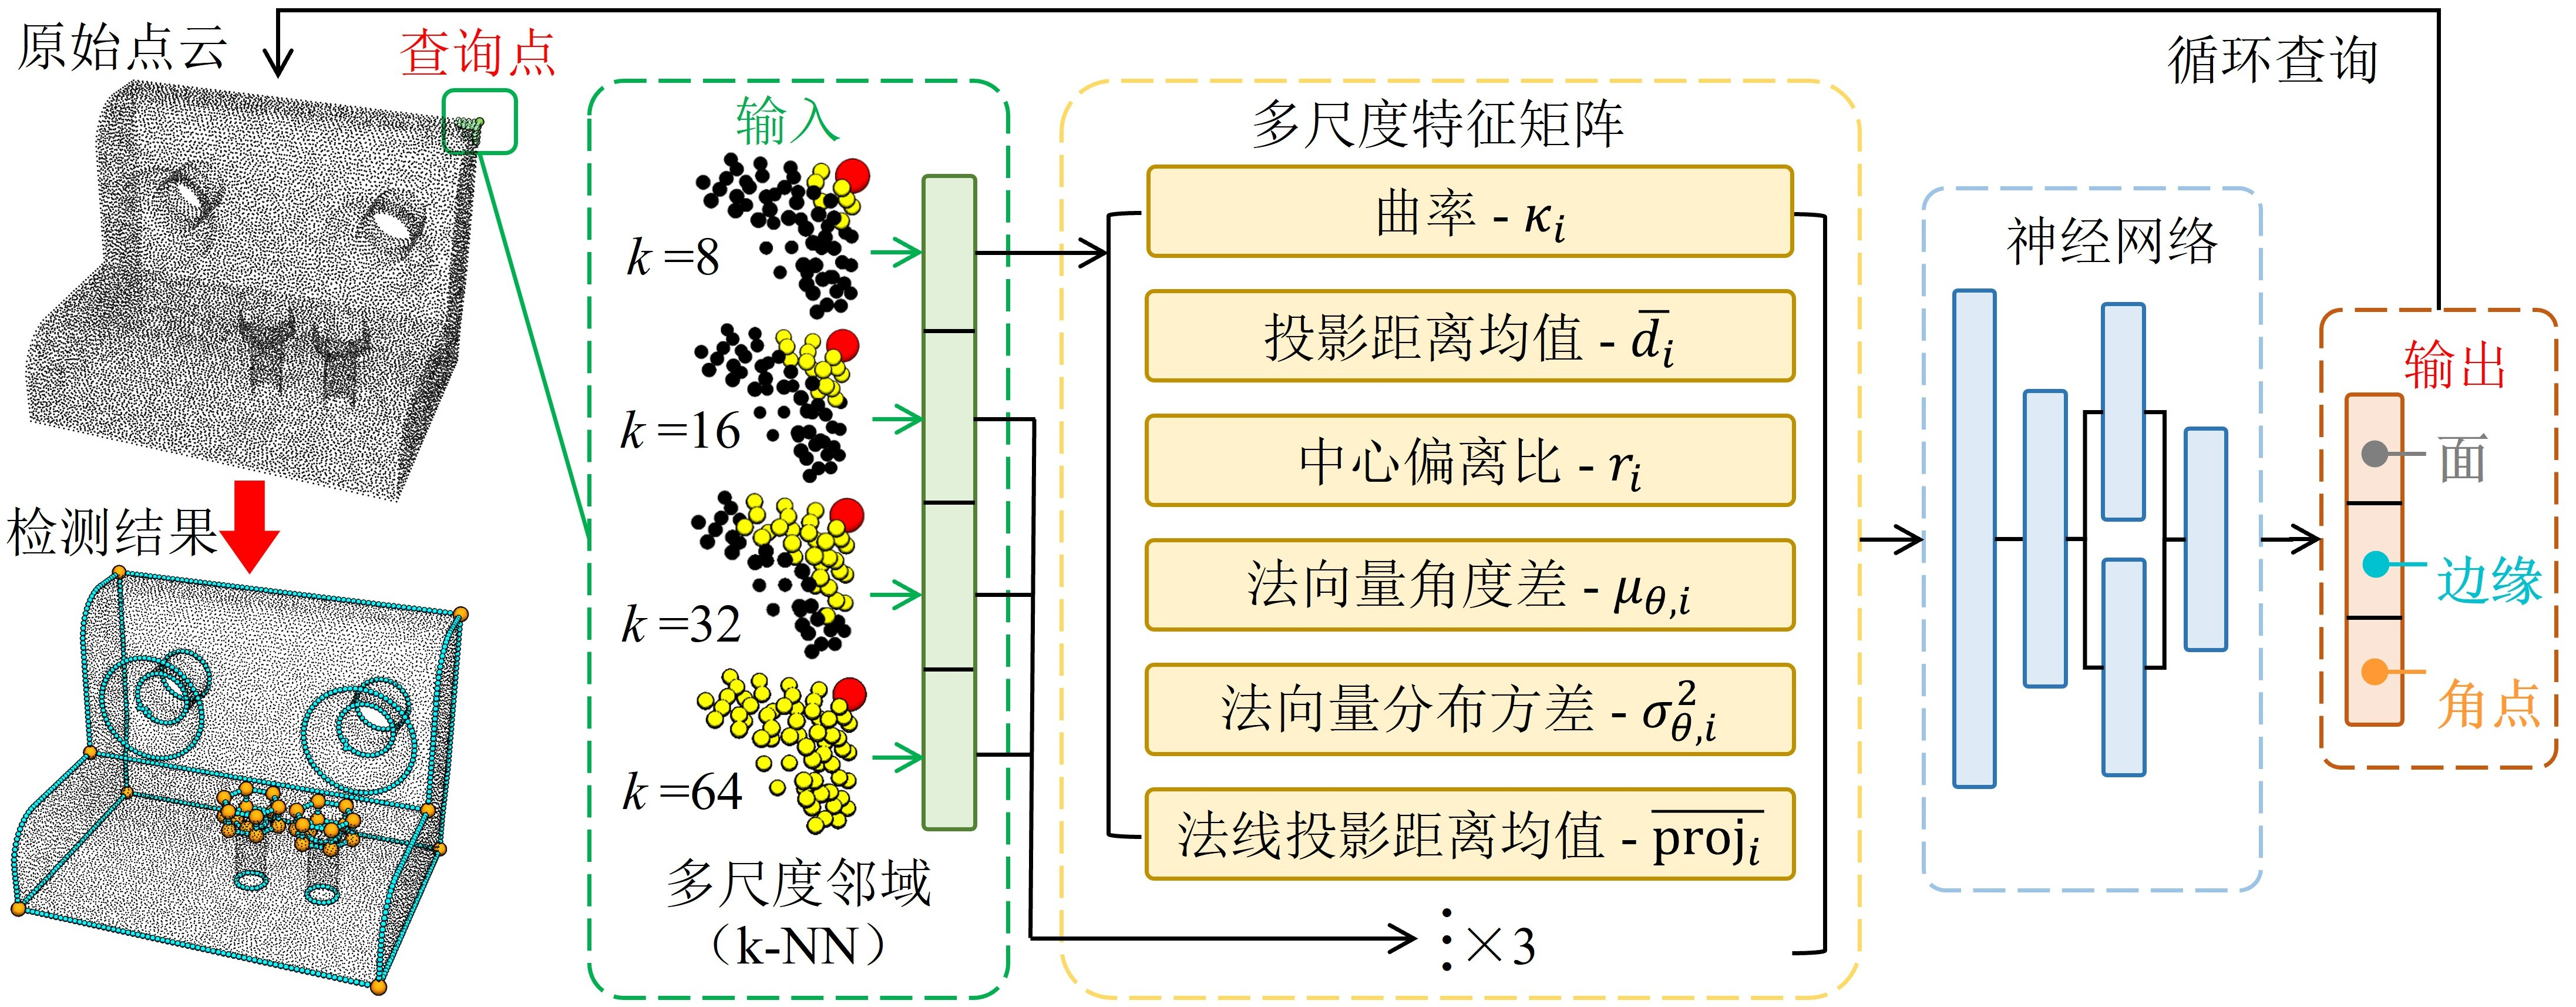
\includegraphics[width=1.0\textwidth]{NECDNet/workflow.jpg}
    \bicaption{NECDNet 网络架构及工作流程示意图。}{NECDNet network architecture and workflow diagram.}
    \label{fig:necdnet_framework}
\end{figure}


\section{多尺度局部特征提取与计算}
多尺度表示的是针对每个查询点，选择不同数量的邻域点以构建多层次的局部几何描述。由于点云捕获时的视角、距离及分辨率等因素影响，单一尺度往往难以全面反映局部几何结构的信息。
通过分析不同尺度下的点云分布特征，可以更全面地捕捉局部几何结构，从而提升边缘和角点的区分能力~\cite{}。适用的尺度取决于多个因素：物体大小、形状复杂度、点云密度、观察尺度等。为了使训练得到的模型能泛化处理未知物体的情况，本文为输入点云中的每个查询点在多尺度邻域内计算多个特征，并在~\ref{cha:xx}进行了消融实验确保各个尺度选择的合理性。

\subsection{多尺度邻域构建}
% 解释 k 近邻搜索与多尺度选择策略。
本文采用基于距离度量的 $k$ 近邻（k-Nearest Neighbors, k-NN）为每个查询点构建多尺度邻域，并以此生成多尺度特征输入网络进行学习~\cite{}。k-NN 是一种基于距离度量的邻域选择方法，通过计算查询点与其他点之间的欧氏距离，选取距离最近的 $k$ 个点作为邻域。与固定半径（radius-based）邻域相比，k-NN 对点云非均匀采样与稀疏区域更加稳健：在稠密区不会过采样、在稀疏区不会因样本不足而破坏特征稳定性。对于非结构化的点云，其只包含点的三维坐标信息，k-NN 方法能够有效适应点云的稀疏性和不均匀分布特性。

为提升检索效率，给定一个非结构化点云 $\mathcal{P}^\text{c} = \{\mathbf{p}_i^\text{c} \mid i = 1, \dots, n\}$，我们在三维坐标空间上构建 KD-树（K-Dimensional Tree）索引~\cite{}。KD-树通过在各坐标轴上递归划分点集，使每个节点对应一个超矩形子空间，从而形成近似平衡的二叉树。查询时，先依据查询点坐标自顶向下定位至叶节点，再在回溯过程中检查可能包含更近邻点的分支，并维护容量为 $k$ 的候选集合以持续更新最近邻。相比于暴力检索的 $O(n)$ 复杂度，KD-树可将单次最近邻查询的平均复杂度降至 $O(\log n)$ ，显著提升大规模点云处理的效率。

基于上述索引结构，对每个查询点 $\mathbf{p}_i^\text{c}$，我们通过 k-NN 方法在点云中搜索其 $k$ 个最近邻点，形成邻域集合 $\mathcal{Q}_i^\text{c} = \{\mathbf{p}_{i,j}^\text{c} \mid j = 1, \dots, k\}$。通过调节 $k$ 的大小即可改变邻域的空间尺度：较小的 $k$ 更敏感于细粒度几何细节（如尖锐小角、细薄边），较大的 $k$ 则能稳健表征更大范围的局部结构。为兼顾不同尺度的几何信息，我们针对多个 $k$ 值为同一查询点构建多组邻域，形成多尺度邻域表示。

具体而言，对由给定 $k$ 值确定的局部区域 $\mathcal{Q}_i^\text{c}$ 计算六个解析特征，得到 6 维特征向量 $\mathbf{x}_i^\text{c}$。当为同一查询点在多个 $k$ 值下重复上述过程，即可获得对应的 $\mathbf{x}_{i,k}^\text{c}$。将这些特征按尺度汇集，构成用于后续网络学习的多尺度特征矩阵，如公式~(\ref{eq:X_i}) 所示：
\begin{equation}
    \mathbf{X}_{i}^\text{c}=\begin{bmatrix}
    \mathbf{x}_{i, k_{1}}^\text{c} \\
    \mathbf{x}_{i, k_{2}}^\text{c} \\
    \vdots \\
    \mathbf{x}_{i, k_{m}}^\text{c}
    \end{bmatrix}
    \label{eq:X_i}
\end{equation}

其中，$k_1, k_2, \ldots, k_m$ 表示所选择的不同邻域尺度，$m$ 为尺度数量。多尺度特征矩阵中的尺度数$m$ 和尺度大小 $k$ 直接影响神经网络的学习结果。具体来说，$k$ 影响结果对点云不同稀疏度的适用性，而 $m$ 影响网络学习数据的维度。选择合适的尺度尺寸和数量可以优化检测精度。因此，在第\ref{}章中，本文对邻近尺度选择进行了消融实验以确定参数，并选择了 $k$ 的四个值：8、16、32和64进行特征计算。

\subsection{局部特征描述符设计}
% 详细介绍位置特征（曲率、投影距离、均值中心距离）和法向量特征（法向角差、法向分布、投影法向模）。

在构建多尺度邻域的基础上，本文进一步设计了一套包含六个维度的局部几何特征描述符，旨在精确捕捉查询点及其邻域在不同空间尺度下的结构属性。这六种特征可归纳为基于位置的几何特征（Position-based Features）与基于法向量方向的特征（Normal-based Features）两大类。
基于位置的特征主要通过分析邻域点的空间分布规律来描述局部形状，而基于法向量的特征则通过分析表面方向的连续性与一致性，提供关于几何边缘与尖锐角点的关键判别信息。这种多维特征的结合，增强了模型在面对复杂、模糊边界时的区分能力。消融实验中对特征计算中涉及的所有描述符进行了评估，说明了该选择的有效性。

\subsubsection{邻域归一化预处理}
% 解释邻域中心化与尺度归一化的步骤与目的。

为了消除点云绝对坐标、平移以及尺度差异对特征计算的影响，在提取特征前，本文首先对邻域 $\mathcal{Q}_i^\text{c}$ 进行归一化处理。该过程基于主成分分析（Principal Component Analysis, PCA）思想，计算邻域点的协方差矩阵 $\mathbf{K}_i = \mathrm{cov}(\mathcal{Q}_i^\text{c})$，并对其进行奇异值分解（Singular Value Decomposition, SVD），如公式(\ref{eq:svd_Ki}) 所示。
\begin{equation}
\mathbf{K}_i = \mathbf{U}_i \boldsymbol{\Sigma}_i \mathbf{V}_i^T
\label{eq:svd_Ki}
\end{equation}

其中，$\mathbf{U}_i$ 和 $\mathbf{V}_i$ 分别为左奇异向量矩阵和右奇异向量矩阵，$\boldsymbol{\Sigma}_i$ 为对角奇异值矩阵。通过该分解，我们能够获得邻域点在主方向上的分布特性。具体而言，通过对角矩阵 $\boldsymbol{\Sigma}_i$ 提取奇异向量 $\boldsymbol{\sigma}_i = (\sigma_{i,1}, \sigma_{i,2}, \sigma_{i,3})$ ，其中的奇异值计为降序排列。右奇异向量矩阵 $\mathbf{V}_i$ 的列向量对应于邻域点在三个主方向上的投影轴。不同的奇异值反映了邻域点在各主方向上的扩展程度。奇异值较小的方向点云分布较为集中，反之则较为分散。
通过上述分解结果，可以对邻域点进行去中心化与尺度归一化处理。具体而言，首先计算邻域点的质心 $\bar{\mathbf{p}}_{i,j}^\text{c}$ ，如公式(\ref{eq:center_Qi})所示。其中$|\mathcal{Q}_i^\text{c}|$ 表示邻域点的数量。
\begin{equation}
    \bar{\mathbf{p}}_{i,j}^\text{c} = \frac{1}{|\mathcal{Q}_i^\text{c}|} \sum_{j=1}^{k} \mathbf{p}_{i,j}^\text{c}
    \label{eq:center_Qi}
\end{equation}22

随后，将所有邻域点坐标减去质心实现去中心化，并利用奇异值 $\sigma_{i,1}$ 和 $\sigma_{i,2}$ 对去中心化后的邻域点进行尺度缩放，确保各个方向上的分布具有统一的量纲，如公式(\ref{eq:norm_Qi})所示。最终，得到归一化后的邻域 $\hat{\mathcal{Q}}_i^\text{c}$，为后续特征计算提供了标准化的输入。归一化邻域后的查询点坐标记为 $\hat{\mathbf{p}}_i^\text{c}$，邻域中的点坐标记为 $\hat{\mathbf{p}}_{i,j}^\text{c}$。
\begin{equation}
    \hat{\mathcal{Q}}_i^\text{c} = \left\{ \frac{2}{\sqrt{\sigma_{i,1}} + 
    \sqrt{\sigma_{i,2}}} \left( \mathbf{p}_{i,j}^\text{c} - \bar{\mathbf{p}}_{i,j}^\text{c} \right) \mid 
    \mathbf{p}_{i,j}^\text{c}\in \mathcal{Q}_i^\text{c} \right\}
    \label{eq:norm_Qi}
\end{equation}

\subsubsection{点云法向量估计}
\label{sec:normal_estimatation}
法向量是描述点云局部表面方位的重要几何属性，也是计算后续方向特征的基础。本文采用基于局部平面拟合的方法估计查询点的法向量。
从公式 (\ref{eq:svd_Ki}) 的奇异值分解结果中可知，奇异值 $\sigma_{i,1}, \sigma_{i,2}, \sigma_{i,3}$ 对应的右奇异向量（即矩阵 $\mathbf{V}_i$ 的列向量）构成了邻域内点集分布的正交主轴。由于奇异值按降序排列，最小奇异值 $\sigma_{i,3}$ 对应的奇异向量 $\mathbf{v}_{i,3}$ 指向了邻域内点集分布方差最小的方向。在几何意义上，该方向与局部最小二乘拟合平面的法向重合。因此，查询点的法向量 $\mathbf{n}_i^\text{c}$ 可直接取为归一化后的右奇异向量 $\mathbf{v}_{i,3}$ 。

然而，仅通过 PCA 获得的法向量存在 $180^\circ$ 的方向模糊性（即法向量可能指向物体内侧或外侧）。为了确保在计算后续法向量夹角差异等特征时的数值一致性，必须对法向量进行定向处理。
在处理具有闭合表面的物体时，通常利用视点方向或邻域一致性进行约束。本文采用最小生成树（Minimum Spanning Tree, MST）算法在点云图中传播法向量方向，以实现全局的方向一致化~\cite{}。具体而言，将点云视为图结构，以点间距离为边权构建图，从初始点开始，通过遍历图确保相邻点的法向量满足内积大于零的约束，实现对点云中各点法向量的方向一致化。

\subsubsection{曲率（ $\kappa_i$ ）}
% 差一张插图
首先计算基于位置的几何特征，表征邻域内点的几何分布特性。曲率 $\kappa_i$ 是几何物体偏离平面程度的度量。在本文中，查询点邻域的曲率可以根据上述得到的奇异值进行计算，用于表征局部表面的平坦程度。具体而言，曲率定义为最大奇异值与三维奇异值之和的比值，如公式(\ref{eq:curvature})所示。
\begin{equation}
    \kappa_i = \frac{\sigma_{i,3}}{\sigma_{i,1} + \sigma_{i,2} + \sigma_{i,3}}
    \label{eq:curvature}
\end{equation}

当查询点位于平坦表面时，$\sigma_{i,3}$ 较小，曲率值接近于零；而当查询点位于尖锐边缘或角点时，$\sigma_{i,3}$ 较大，曲率值相应增大。因此，曲率特征有助于区分面点与边缘、角点。

\subsubsection{投影距离均值（ $\bar{d_i}$ ）}
% 差一张插图
投影距离均值 $\bar{d_i}$ 用于刻画查询点邻域内点相对于该点法向平面的空间分布，其大小反映了局部几何结构的突变程度。具体地，对于任一查询点 $\hat{\mathbf{p}}_i^\text{c}$，结合其法向量 $\mathbf{n}_i^\text{c}$ 可定义通过该点的投影平面。邻域内所有点 $\hat{\mathbf{p}}_{i,j}^\text{c}$ 到该投影平面的距离均值即为 $\bar{d}_i$，计算公式如(\ref{eq:projection_distance})所示。
\begin{equation}
    \bar{d}_i = \frac{1}{|\hat{\mathcal{Q}}_i^\text{c}|} \sum_{\hat{\mathbf{p}}_{i,j}^\text{c} \in \hat{\mathcal{Q}}_i^\text{c}} \left| (\hat{\mathbf{p}}_{i,j}^\text{c} - \hat{\mathbf{p}}_i^\text{c}) \cdot \mathbf{n}_i^\text{c} \right|
    \label{eq:projection_distance}
\end{equation}

图~\ref{}展示了该距离度量的几何意义。其反映了邻域点在查询点法向方向上的分布特性：当邻域点主要分布在查询点法向平面附近时，投影距离较小，表明局部几何结构较为平滑；而当邻域点在法向方向上分布较为分散时，投影距离增大，通常对应于边缘或角点区域。

\subsubsection{中心偏离比（ $r_i$ ）}
中心偏离比 $r_i$ 是量化查询点在其局部邻域内的相对空间位置的度量，其能够衡量查询点相对于其邻域质心的偏移程度。具体而言，首先计算邻域点的质心，由于此时的邻域 $\hat{\mathcal{Q}}_i^\text{c}$ 已经进行了去中心化及归一化处理，因此邻域质心即为原点。之后计算查询点到质心的距离 $\| \hat{\mathbf{p}}_i^\text{c} \|$ 与邻域内各点到质心距离 $\| \hat{\mathbf{p}}_{i,j}^\text{c}\|$ 的最小值之比，得到中心距离均值比 $r_i$，计算公式如(\ref{eq:mean_center_distance})所示，由于该特征为比值，当分母较小时产生的结果不受此前归一化邻域的影响。故针对特征 $r_i$，本文选用 Sigmoid 函数对其进行标准化处理，以减小数值分布的变化范围。
\begin{equation}
    r_i = \operatorname{Sigmoid}\left(\frac{\| \hat{\mathbf{p}}_i^\text{c} \|}{\min_{\hat{\mathbf{p}}_{i,j}^\text{c} \in \hat{\mathcal{Q}}_i^\text{c}} \| \hat{\mathbf{p}}_{i,j}^\text{c}\|}\right)
    \label{eq:mean_center_distance}
\end{equation}

其中 $\operatorname{Sigmoid}$ 表示 Sigmoid 函数，$\| \cdot \|$ 表示欧氏距离，$\min$ 运算符用于获取邻域点中距离质心最近的点的距离，式中省略了减去质心零向量的表示。中心偏离比 $r_i$ 反映了查询点在邻域内的相对位置关系：当查询点位于邻域质心附近时，$r_i$ 值较小，表明该点可能位于平坦区域；而当查询点远离邻域质心时，$r_i$ 值增大，通常对应于边缘或角点区域。因此，中心偏离比有助于区分不同几何特征。

\subsubsection{法向量角度差（$\mu_{\theta,i}$）}
以此特征描述符开始，后续的三个描述符是基于法向量方向的特征，旨在捕捉表面方向的突变信息。法向角度差 $\mu_{\theta,i}$ 衡量查询点法向量与其邻域内各点法向量之间夹角的平均值，反映了局部表面方向的一致性。具体而言，首先根据章节\ref{sec:normal_estimatation}中的方法估计邻域内每个点的单位法向量 $\mathbf{n}_{i,j}^\text{c}$，组合为 $\mathcal{N}_i^\text{c}$。随后，计算查询点法向量 $\mathbf{n}_i^\text{c}$ 与邻域内各点法向量之间的夹角 $\theta_{i, j}$ ，计算公式如(\ref{eq:normal_angle})。最后并求各个夹角的平均值，求解公式如(\ref{eq:normal_angle_difference})所示。
\begin{equation}
    \theta_{i,j} = \arccos \left( \mathbf{n}_i^\text{c} \cdot \mathbf{n}_{i,j}^\text{c} \right)
    \label{eq:normal_angle}
\end{equation}
\begin{equation}
    \mu_{\theta,i} = \frac{1}{|\mathcal{N}_i^\text{c}|} \sum_{j=1}^{|\mathcal{N}_i^\text{c}|} \theta_{i,j}
    \label{eq:normal_angle_difference}
\end{equation}

其中，$\arccos$ 表示反余弦函数。法向角度差 $\mu_{\theta,i}$ 反映了邻域内法向量的方向变化程度：当邻域内法向量与查询点法向量高度一致时，$\mu_{\theta,i}$ 值较小，表明局部表面较为平滑；而当邻域内法向量与查询点法向量差异较大时，$\mu_{\theta,i}$ 值增大，通常对应于边缘或角点区域。

此外，除了用法向量夹角来表示方向变化外，还可以直接使用法向量的数值之差来表示方向变化。具体而言，计算查询点法向量与邻域内各点法向量的差值，并求其平均值，得到法向量数值差 $\bar{\Delta \mathbf{n}}_i$，计算公式如(\ref{eq:normal_value_difference})所示。相较与法向量角度差 $\mu_{\theta,i}$，法向量数值差 $\bar{\Delta \mathbf{n}}_i$ 直接采用原始法向量数据进行统计计算，后续消融实验中会讨论两者的效果差异。
\begin{equation}
    \bar{\Delta \mathbf{n}}_i = \frac{1}{|\mathcal{N}_i^\text{c}|} \sum_{\mathbf{n}_{i,j}^\text{c} \in \mathcal{N}_i^\text{c}} ( \mathbf{n}_i^\text{c} - \mathbf{n}_{i,j}^\text{c} )
    \label{eq:normal_value_difference}
\end{equation}

\subsubsection{法向量分布方差（ $\sigma^2_{\theta,i}$ ）}
法向量分布方差 $\sigma^2_{\theta,i}$ 用于量化邻域内法向量夹角的变化剧烈程度，反映了局部表面方向的稳定性。具体而言，基于前述计算的法向角度差 $\mu_{\theta,i}$，计算邻域内各点法向量与查询点法向量夹角的方差，求解公式如(\ref{eq:normal_distribution_variance})所示。
\begin{equation}
    \sigma^2_{\theta,i} = \frac{1}{|\mathcal{N}_i^\text{c}|} \sum_{j=1}^{|\mathcal{N}_i^\text{c}|} (\theta_{i,j} - \mu_{\theta,i})^2
    \label{eq:normal_distribution_variance}
\end{equation}

法向量分布方差 $\sigma^2_{\theta,i}$ 反映了邻域内法向量变化的剧烈程度：当邻域内法向量夹角较为集中时，$\sigma^2_{\theta,i}$ 值较小，表明局部表面方向较为稳定；而当邻域内法向量夹角分布较为分散时，$\sigma^2_{\theta,i}$ 值增大，通常对应于边缘或角点区域，而角点区域的分散程度更为显著。

\subsubsection{法线投影距离均值（ $\bar{\text{proj}_i}$ ）}
法线投影距离均值 $\bar{\text{proj}_i}$ 用于量化邻域点法向量在查询点法向上的投影强度，反映了表面法向的对齐程度。具体而言，计算邻域内每个点法向量 $\mathbf{n}_{i,j}^\text{c}$ 在查询点法向 $\mathbf{n}_i^\text{c}$ 上的投影长度，并求其平均值，计算公式如(\ref{eq:projectional_normal_norm})所示。
\begin{equation}
    \bar{\text{proj}_i} = \frac{1}{|\mathcal{N}_i^\text{c}|} \sum_{\mathbf{n}_{i,j}^\text{c} \in \mathcal{N}_i^\text{c}} \left| \mathbf{n}_{i,j}^\text{c} \cdot \mathbf{n}_i^\text{c} \right|
    \label{eq:projectional_normal_norm}
\end{equation}

由于各点的法向量均为单位向量，法线投影距离均值 $\bar{\text{proj}_i}$ 可以反映邻域内法向量与查询点法向量的对齐程度：$\bar{\text{proj}_i}$ 值较大，表明局部表面方向较为统一；而当邻域内法向量与查询点法向量差异较大时，$\bar{\text{proj}_i}$ 值减小，通常对应于边缘或角点区域。

\subsection{局部特征描述符数值可视化分析}
% 展示不同特征在区分面、边、角时的分布差异。
通过上述计算的局部特征描述符，本文最终选择了其中六个组成特征描述向量，并用于后续的特征融合和分类任务。最后得到的特征向量如公式(\ref{eq:feature_vector})所示。六个特征均为标量，组成的特征向量维度为 6，包含了点云的位置分布特性和法向量变化信息，能够有效表征点云局部的几何结构属性。
\begin{equation}
    \mathbf{x}_i^\text{c} = \left( \kappa_i, \bar{d}_i, r_i, \mu_{\theta,i}, \sigma^2_{\theta,i}, \bar{\text{proj}_i} \right)
    \label{eq:feature_vector}
\end{equation}

图~\ref{fig:feature_distribution} 展示了多尺度几何特征在点云三类特征（面、边缘、角点）中的分布表现，直观体现了所选六维特征向量对于区分不同几何类别的有效性。
其中图(a)对单个物体点云的六个特征进行了空间分布可视化。每个子图分别显示了特征描述符 $\kappa_i$（曲率）、$\bar{d}_i$（投影距离均值）、$r_i$（中心偏离比）、$\mu_{\theta,i}$（法向量角度差）、$\sigma^2_{\theta,i}$（法向量分布方差）、$\bar{\text{proj}_i}$（法向投影距离均值）在点云空间上的数值分布情况。颜色表示数值大小，采用从蓝色（低值）到红色（高值）的渐变色带。根据上一小节对各特征的定义，可以观察到：除了特征$\bar{\text{proj}_i}$外，其他五个特征在面、边缘和角点区域均表现出从低到高的数值变化趋势（蓝色到红色）。而特征$\bar{\text{proj}_i}$ 则呈现出相反的趋势，在面区域数值较高（红色），而在边缘和角点区域数值降低（橙黄色）。各个特征在不同的几何结构上有着明显的区别。

图(b)部分给出了在我们构建的数据集ABC-Corner中1000个点云样本的六个特征在三类标签下的数值分布，数据集的描述及构建过程请见章节(\ref{sec:dataset})。纵轴为点云ID，横轴为特征值，颜色标记类别：蓝色为面、黄色为边缘、红色为角点。统计结果显示，在面、边缘、角点三类之间，所有特征分布具有明显的界限。
以曲率和法向分布为例，角点（红色）主要集中在中高值段，面点则聚集于低值，边缘点分布于中间区域。其他如投影距离、均值中心距离等特征也展现出对类别的良好区分能力。

虽然可以观察到直接使用这些特征描述符就能进行一定程度上的几何特征区分。然而，直接使用这些特征进行检测类似于分析方法，需要参数调整并且可能无法保证稳健的结果。为了解决这个问题，本文利用神经网络从计算的特征矩阵中学习。这种方法使能够结合分析方法和基于学习的检测技术的优势，实现精准的自分类。
\begin{figure}
    \centering
    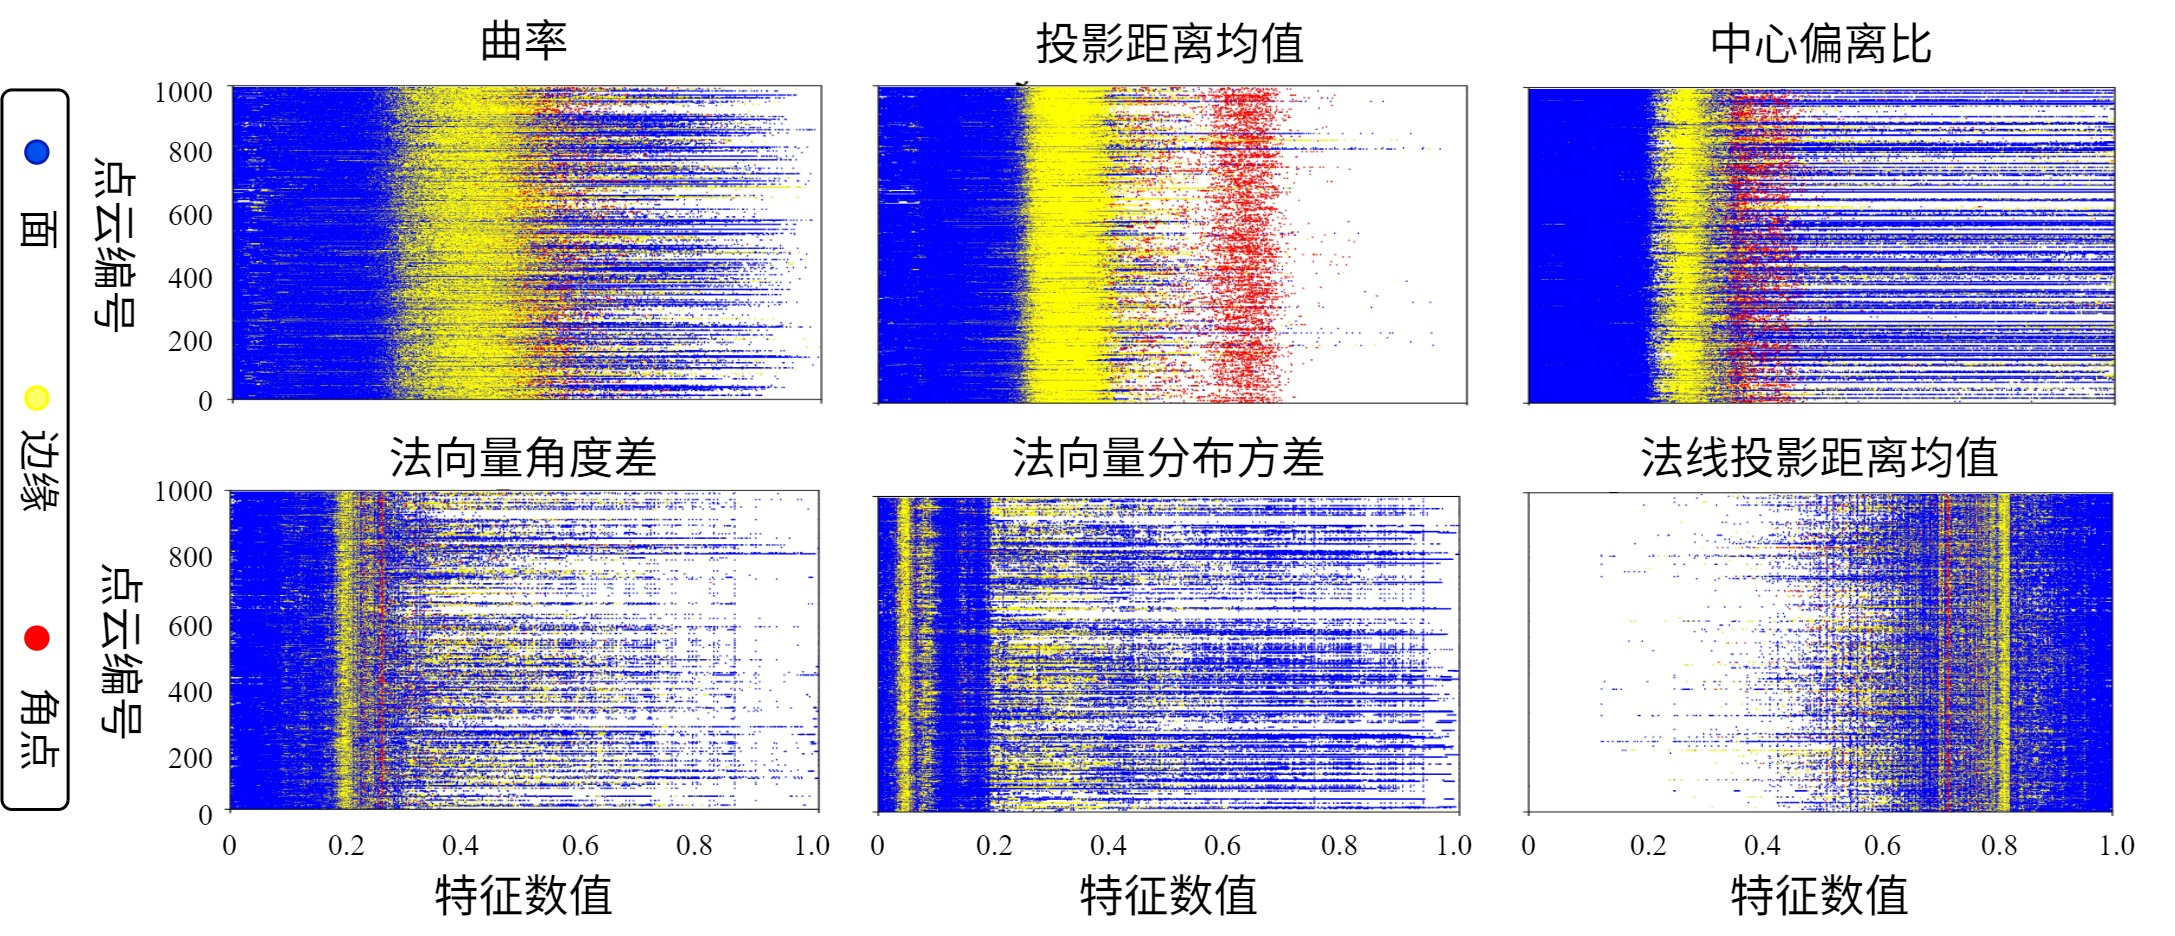
\includegraphics[width=1.0\textwidth]{NECDNet/feature_distribution.jpg}
    \bicaption{六个局部特征描述符在不同几何类别下的数值分布情况。}{Distribution of six local feature descriptors across different geometric categories.}
    \label{fig:feature_distribution}
\end{figure}


\section{\textrm{NECDNet} 网络架构设计}
% 阐述 MLP 基础的层次化网络结构。
% 多尺度特征矩阵的构建与输入。
% 分类器的设计与Dropout策略防止过拟合。
NECDNet 的网络架构设计基于多层感知机（Multi-Layer Perceptron, MLP）结构，旨在通过逐层融合多尺度局部特征矩阵，实现对点云中面点、边缘点和角点的高精度分类。该网络架构充分利用了前述计算的多尺度特征矩阵，结合深度学习的强大表达能力，有效捕捉点云局部几何结构的复杂关系。

图~\ref{fig:necdnet_architecture} 展示了 NECDNet 的具体网络结构。网络的输入为 $n$ 个查询点的多尺度特征矩阵 $\mathbf{X}_i^\text{c}$，其维度为 $n \times m \times 6$，其中 $m$ 为尺度数量（本文中取4）。网络整体可以分为两个本部分：多尺度特征融合及逐级分类。网络由多个全连接层（绿色）组成，每层后均采用 Leaky ReLU 激活函数（红色）以引入非线性变换，从而增强模型的表达能力。为了防止过拟合，网络中还引入了 Dropout 层（蓝色），在训练过程中随机丢弃部分神经元连接，提升模型的泛化能力。网络的输出为在，面、边缘、角点，三个类别上的分数，通过 Softmax 函数进行归一化获得，在三个类别中数值最大的类别即为最终的分类结果。
\begin{figure}[!htbp]
    \centering
    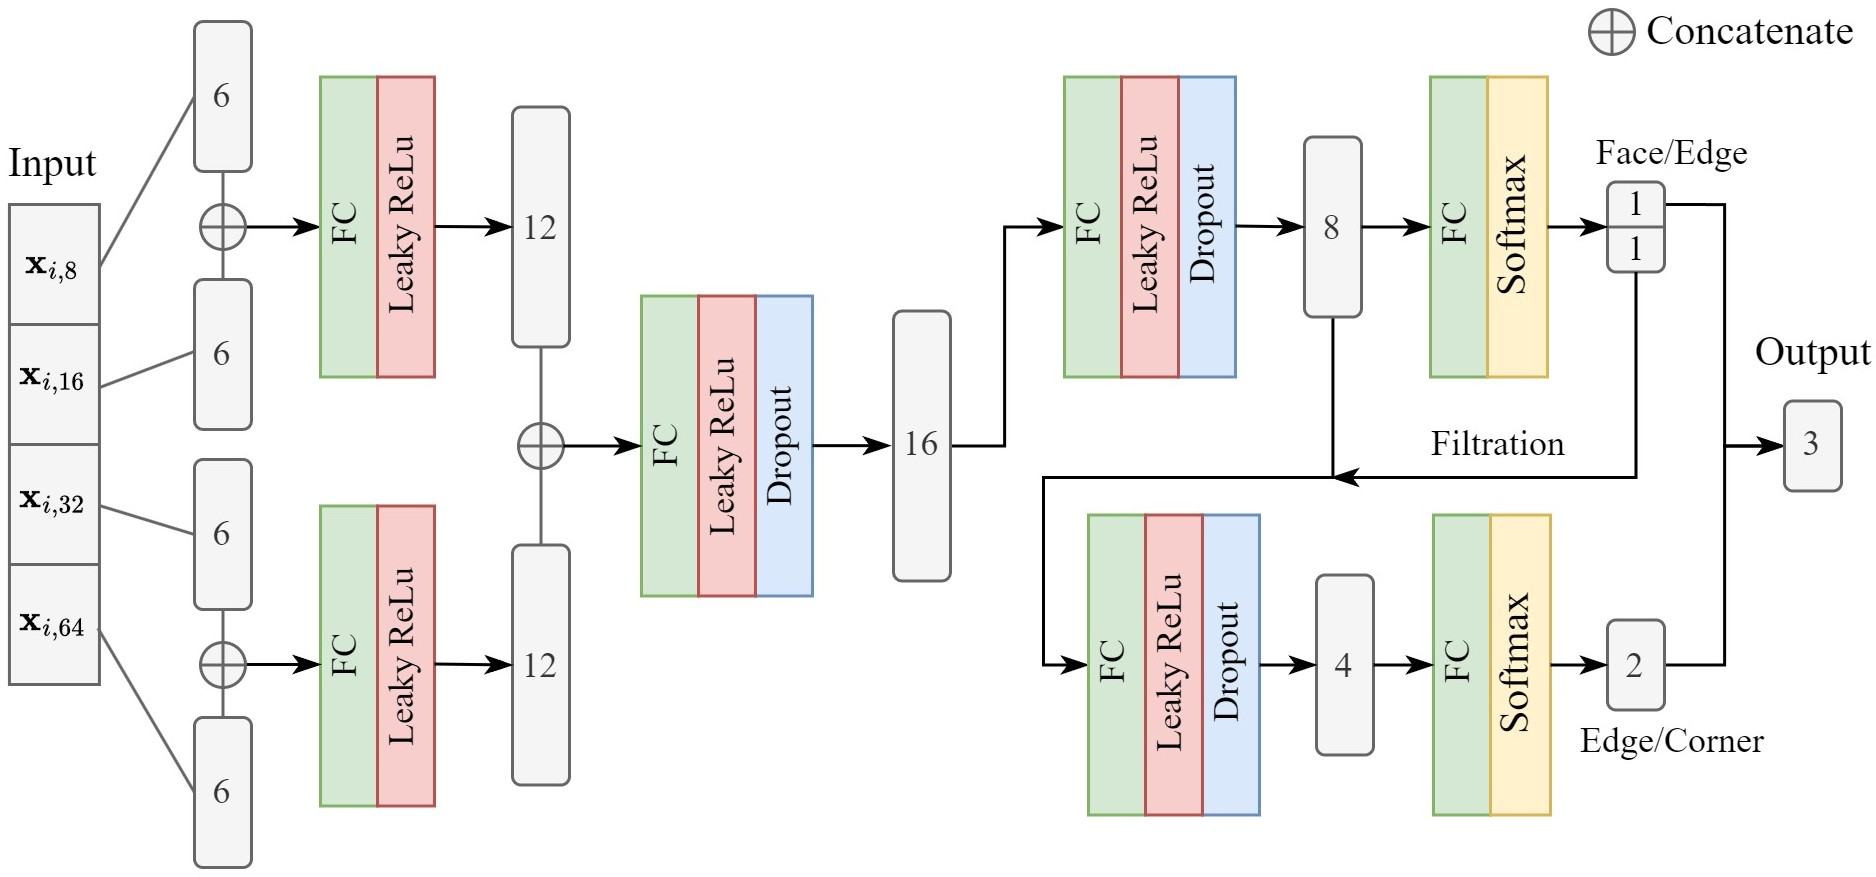
\includegraphics[width=1.0\textwidth]{NECDNet/necdnet_architecture.jpg}
    \bicaption{NECDNet 网络架构示意图。}{NECDNet network architecture diagram.}
    \label{fig:necdnet_architecture}
\end{figure}

\subsection{多尺度特征融合}
由于网络输入的数据是在多个邻域尺度下得到的，各个尺度下的特征矩阵包含了不同层次的局部几何信息。如果只是进行简单的拼接或平均处理，可能无法充分利用各尺度间的互补信息。因此，NECDNet 设计了逐层融合的机制，通过多层感知机对各尺度特征进行逐级整合，将特征的融合也作为网络的一部分进行学习。

具体而言，本文中输入的单个查询点的特征矩阵 $\mathbf{X}_i^\text{c}$ 包含四个尺度（$k=8,16,32,64$）下的六维特征。网络采用两两融合的方式，将输入的四个尺度的特征进行两两拼接（8和16，32和64）。随后，通过全连接层对拼接后的特征进行非线性变换和降维处理，得到融合后的特征向量，融合后的向量维度为 12。第二层对融合后的特征再次进行两两拼接，并通过全连接层进行进一步的融合和降维，最终得到一个 16 维的特征向量。其中降维到16是为了减轻后续的计算，使网络更加轻量化。此外，在进行非线性变换后，为了防止过拟合的现象，本文引入了Dropout层。最终的融合向量综合了不同尺度下的局部几何信息，为后续的分类任务提供了丰富的输入。

\subsection{逐级分类器}
特征融合后则进入逐级分类器部分。与特征融合类似，该部分也主要由全连接层组成，采用 Leaky ReLU 激活函数。但在具体结构上，逐级分类器部分使用分层设计，首先进行简单的分类任务（面、非面点），根据结果过滤非面点再进行更细粒度的分类（边缘、角点）。这种设计有助于简化分类任务，提高整体的分类准确率。

具体而言，首先让维度 16 的融合特征通过一个全连接层，输出维度为 8 的中间特征向量。随后，该中间特征向量通过另一个全连接层，输出维度为 2 的面、非面分类分数。根据该分数，本文采用阈值过滤的方式，将非面点送入下一级分类器进行边缘、角点的细粒度分类。下一级分类器同样由两个全连接层组成，首先将维度 8 的中间特征向量通过一个全连接层，输出维度为 4 的特征向量。随后，该特征向量通过另一个全连接层，输出维度为 2 的边缘、角点分类分数。最终，通过 Softmax 函数对三个分类分数进行归一化处理，得到每个类别的概率分布。
\subsection{损失函数}
点云中几何特征的分布存在不平衡现象，面点数量远多于边缘点和角点，特别是角点。为了应对类别不平衡问题，本文在训练过程中采用 Focal Loss 作为优化指标~\cite{}。该损失函数通过为不同类别分配不同的权重，增强对少数类别（边缘点和角点）的关注，从而提升模型在这些类别上的识别能力。

\subsection{评价指标}

\section{\textrm{ABC-Corner} 数据集构建}
\label{sec:dataset}
\subsection{数据集模型选取}
\subsection{初步标注}
\subsection{r}
% 介绍数据集来源（ABC dataset）及筛选标准。
% 详述标注流程（从CAD模型提取边缘 -> 几何规则提取粗角点 -> 人工精修）。
% 数据集的统计特性与类别不平衡处理（过采样策略）。

\section{本章小结}
% !Mode:: "TeX:UTF-8"
\chapter{考虑边缘与角点接触的机器人抓取规划}
\label{cha:theorem}
\section{引言}

\section{基于几何特征的接触点采样与配对}
\subsection{类别感知的体素采样}
% 针对面、边、角不同区域的均衡采样策略。
\subsection{特征化接触检测器设计}
% 面接触：圆柱体检测器。
% 边接触：扇形柱检测器。
% 角接触：圆锥体检测器。
\subsection{对偶接触点配对策略}
% 基于法向量约束和几何位置的筛选规则。

\section{基于软接触模型的稳定性评估}
% 软指接触变形假设与接触区域建模（参数 η ）。
% 摩擦力约束与力平衡方程构建。
% 抓取配置生成与碰撞检测。

\section{抓取增强策略}
% 沿接触向量的旋转增强（Grasp augmentation）。

\section{本章小结}

% !Mode:: "TeX:UTF-8"
\chapter{实验结果与分析}
\section{实验环境及配置}
% 硬件平台（GPU、机械臂型号、手爪参数）。
% 软件环境与评价指标（Precision, Recall, F1, Success Rate, 抓取分布统计指标）。

\section{点云特征检测实验分析}
\subsection{对比实验}
% 与 PIE-Net, PCEDNet, BoundED 等 SOTA 方法在 ABC-Corner 数据集上的对比（重点展示角点检测的优越性）。
\subsection{消融实验}
% 特征维度选择的影响、邻域尺度数量的影响、过采样策略的有效性。
\subsection{结果可视化}
% 展示不同物体点云的边缘与角点分割效果。

\section{抓取规划仿真实验分析}
\subsection{抓取分布多样性评估}
% 引入标准差(STD)、极差(R)等指标，对比本文方法与 GraspIt!, GPD, WRS 的抓取空间覆盖能力。
\subsection{典型物体抓取规划结果}
% 针对四面体、不规则棱柱、日用品等物体的规划结果展示（突出六种接触组合）。
\subsection{参数敏感性分析}
% 采样体素大小、检测器角度阈值等参数对规划结果的影响。

\section{真实机器人抓取实验}
% 实验设置与流程（物体放置、运动规划、抓取执行）。
% 多类别物体（工业件、日用品、异形件）的抓取成功率统计。
% 对边缘和角点接触抓取的实际效果验证。
\section{本章小结}

\chapter{机器人抓取规划实验结果及分析}
\label{ch:experiments}

本章通过仿真和真实抓取实验验证所提规划方法。实验分为两部分：首先比较不同方法生成抓取构型的分布特性；随后在真实机器人平台上统计抓取成功率。最后讨论方法的适用范围与局限性。

\section{实验环境及配置}
\label{sec:exp_setup}

\subsection{真实环境}
真实实验平台由 ABB GOFA-5 机械臂与 DH-ROBOTICS PGC 平行夹爪组成。夹爪最大行程为 76 mm，通过更换手指可分别配置为 0 到 76 mm 或 30 到 106 mm 两种开口范围；指腹为直径 28 mm、厚度 3 mm 的圆形垫片，摩擦系数约为 0.25。

实验共使用 9 个物体，包含开源数据集模型、工业件与日用品，并加入人工设计的四面体以测试极端几何场景。样本选择原因见附录 IV。

\begin{figure}[htbp]
    \centering
    % 请替换为实际图片文件名
    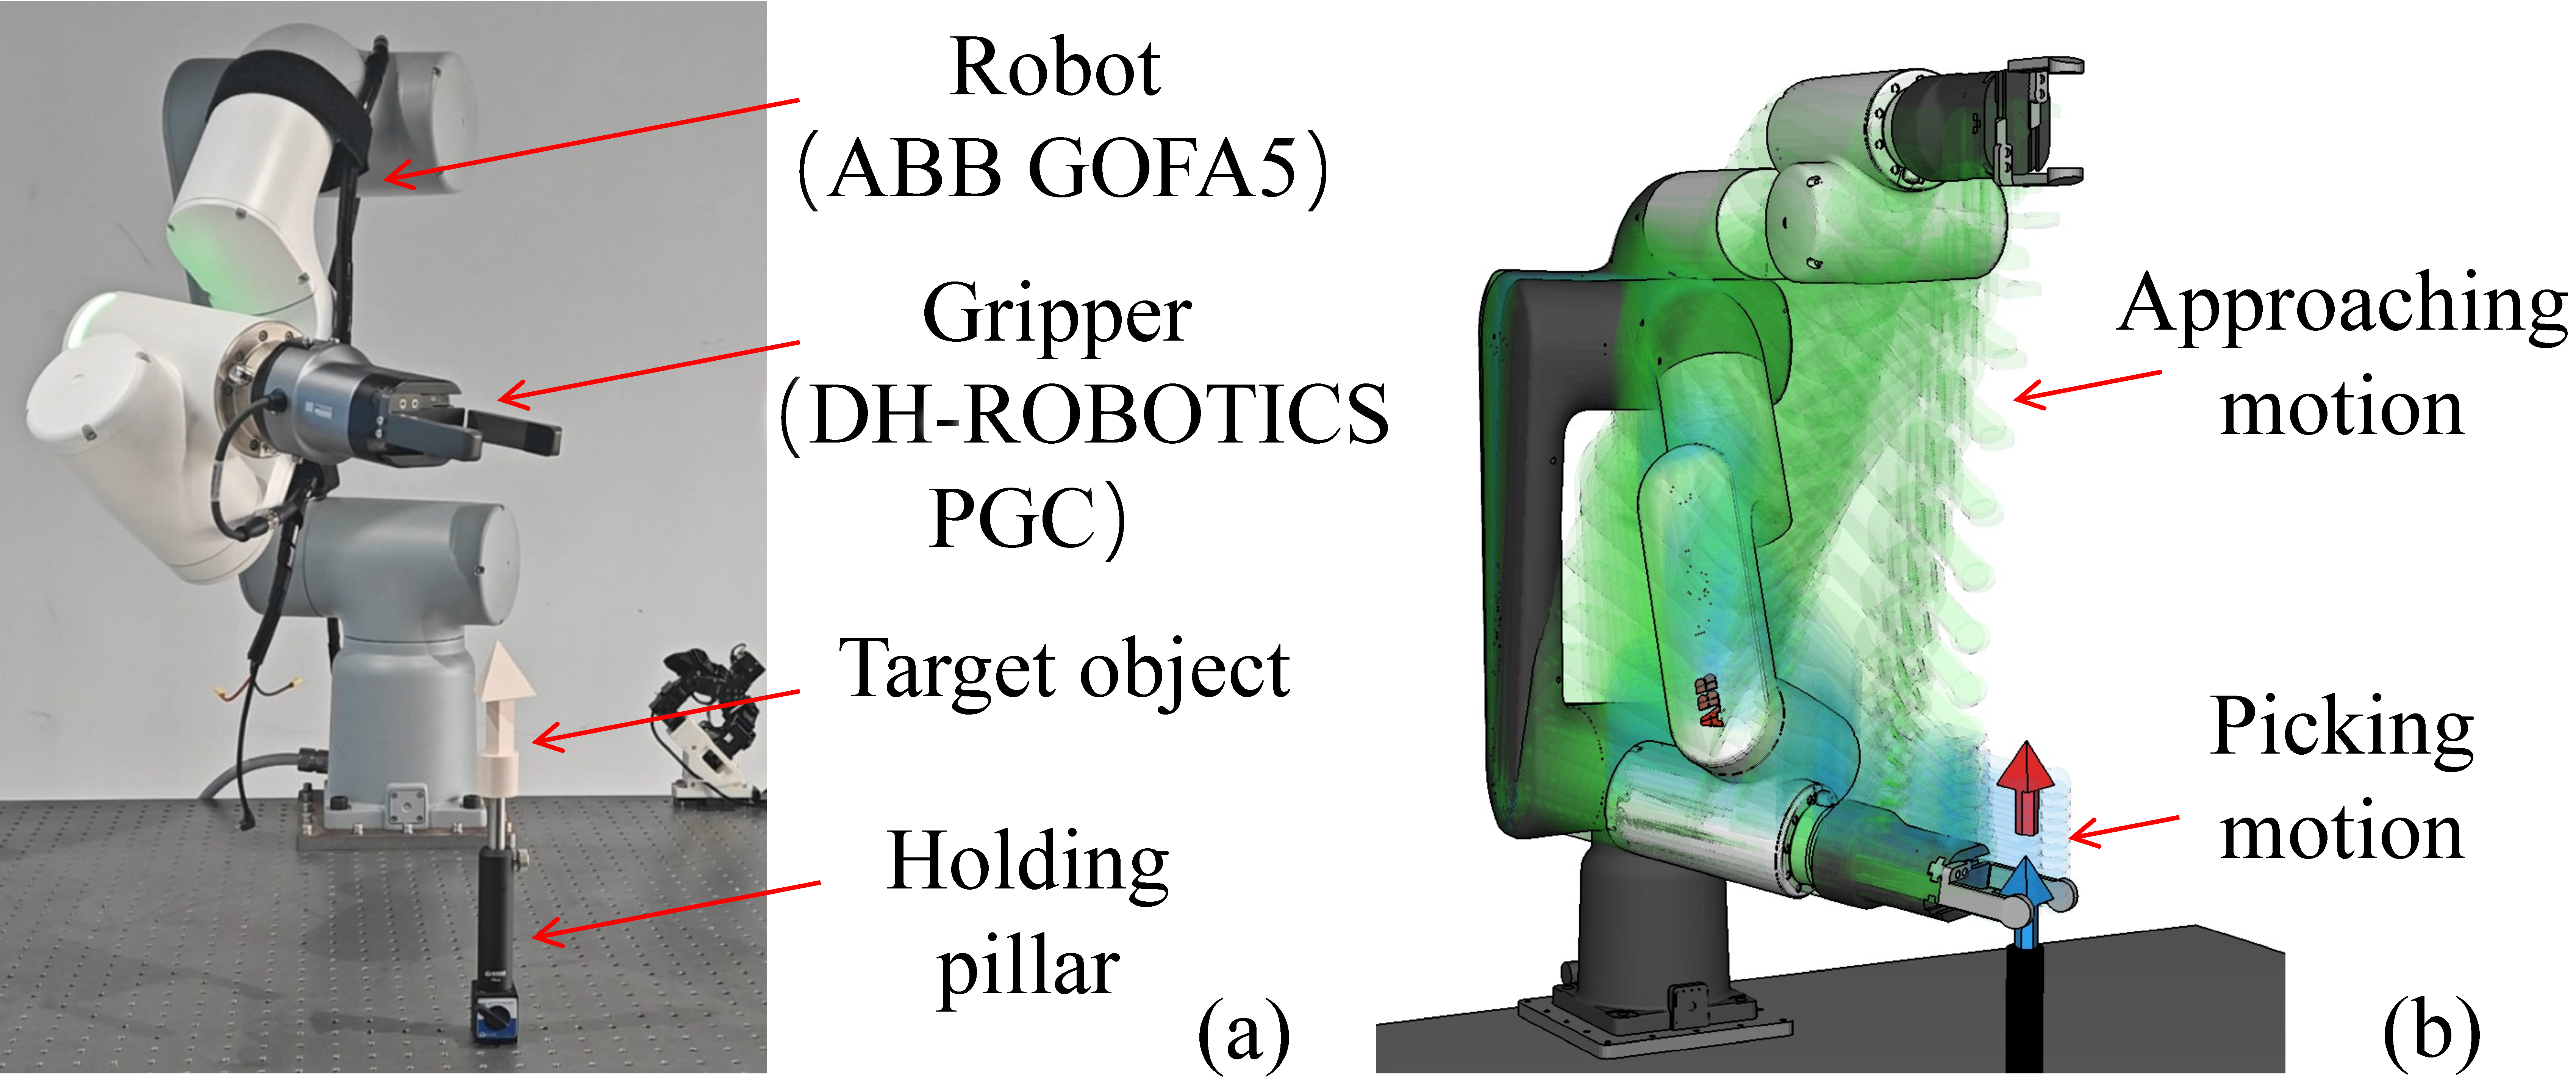
\includegraphics[width=0.8\linewidth]{FBGrasp/setting.pdf}
    \caption{(a) 真实物理实验场景设置；(b) 机器人运动规划路径示意：接近物体（绿色）、执行抓取（蓝色）及移动至目标位（绿色）。}
    \label{fig:setting}
\end{figure}

\subsection{仿真环境}
仿真实验用于定量分析抓取分布。为保证公平性，实验中物体位姿设为已知真值，不引入视觉误差。对比方法包括 GraspIt!、GPD 与 WRS，三者均在相同计算条件下运行。

\section{抓取分布多样性对比}
\label{sec:distribution_comparison}

\subsection{抓取分布统计指标}
除稳定性与可抓取性外，本文将抓取构型分布作为重要评价标准。分布越广、越均匀，机器人在复杂环境中的接近与执行灵活性越高。

具体地，统计对象为抓取构型的 6D 数据，并重点分析接触向量 $\mathbf{v}_i$。采用三个指标：标准差（STD）、极差（R）与平均绝对偏差（MAD）。为消除候选数量差异，每种方法均先生成超过 20 个候选，再统一降采样为 20 个。定量比较对象为四面体、Amicelli 和 Seal。

% 添加表格：分布指标对比
\begin{table}[htbp]
    \centering
    \small
    \setlength{\tabcolsep}{5pt}
    \caption{不同抓取规划方法在三个测试物体上的分布统计指标对比}
    \label{tab:distribution_metrics}
    \begin{threeparttable}
    \begin{tabular}{lcccc}
        \toprule
        \textbf{物体} & \textbf{方法} & \textbf{STD ($\uparrow$)} & \textbf{R ($\uparrow$)} & \textbf{MAD ($\uparrow$)} \\
        \midrule
        \multirow{4}{*}{四面体} 
        & GraspIt!~\cite{miller_graspit_2021} & 0.2516 & 0.8676 & 0.1998 \\
        & GPD~\cite{ten2017grasp} & 0.2878 & 0.9375 & 0.2389 \\
        & WRS~\cite{wan2020planning} & / & / & / \\
        & \textbf{本文方法} & \textbf{0.2995} & \textbf{0.9498} & \textbf{0.2450} \\
        \midrule
        \multirow{4}{*}{巧克力（Amicelli）} 
        & GraspIt!~\cite{miller_graspit_2021} & 0.1669 & 0.6687 & 0.1177 \\
        & GPD~\cite{ten2017grasp} & 0.2742 & 0.9454 & 0.2162 \\
        & WRS~\cite{wan2020planning} & 0.2639 & 0.9365 & 0.2002 \\
        & \textbf{本文方法} & \textbf{0.2835} & \textbf{0.9922} & \textbf{0.2193} \\
        \midrule
        \multirow{4}{*}{海豹（Seal）}
        & GraspIt!~\cite{miller_graspit_2021} & 0.2718 & 0.9063 & 0.2154 \\
        & GPD~\cite{ten2017grasp} & 0.2667 & 0.8409 & 0.2284 \\
        & WRS~\cite{wan2020planning} & 0.2427 & 0.8690 & 0.2014 \\
        & \textbf{本文方法} & \textbf{0.2857} & \textbf{0.9154} & \textbf{0.2429} \\
        \bottomrule
    \end{tabular}
    \begin{tablenotes}
        \footnotesize
        \item STD：标准差；R：极差；MAD：平均绝对偏差。
        \item WRS 对四面体无法生成有效抓取候选，以"/"表示。
    \end{tablenotes}
    \end{threeparttable}
\end{table}

\subsection{抓取分布可视化}
表 \ref{tab:distribution_metrics} 显示，本文方法在三个对象上的 STD、R、MAD 均为最优，说明生成的候选抓取覆盖范围更大、方向更分散。

图 \ref{exp:distribution}(a) 的夹爪可视化也支持这一结论。与主要依赖面接触的方法相比，本文方法可利用边缘与角点接触，在四面体等几何受限物体上仍能生成可行且多样的抓取。图 \ref{exp:distribution}(b) 的三维散点图进一步表明，本文方法在姿态空间中覆盖更广且分布更均匀。

\begin{figure}[htbp]
    \centering
    % 请替换为实际图片文件名
    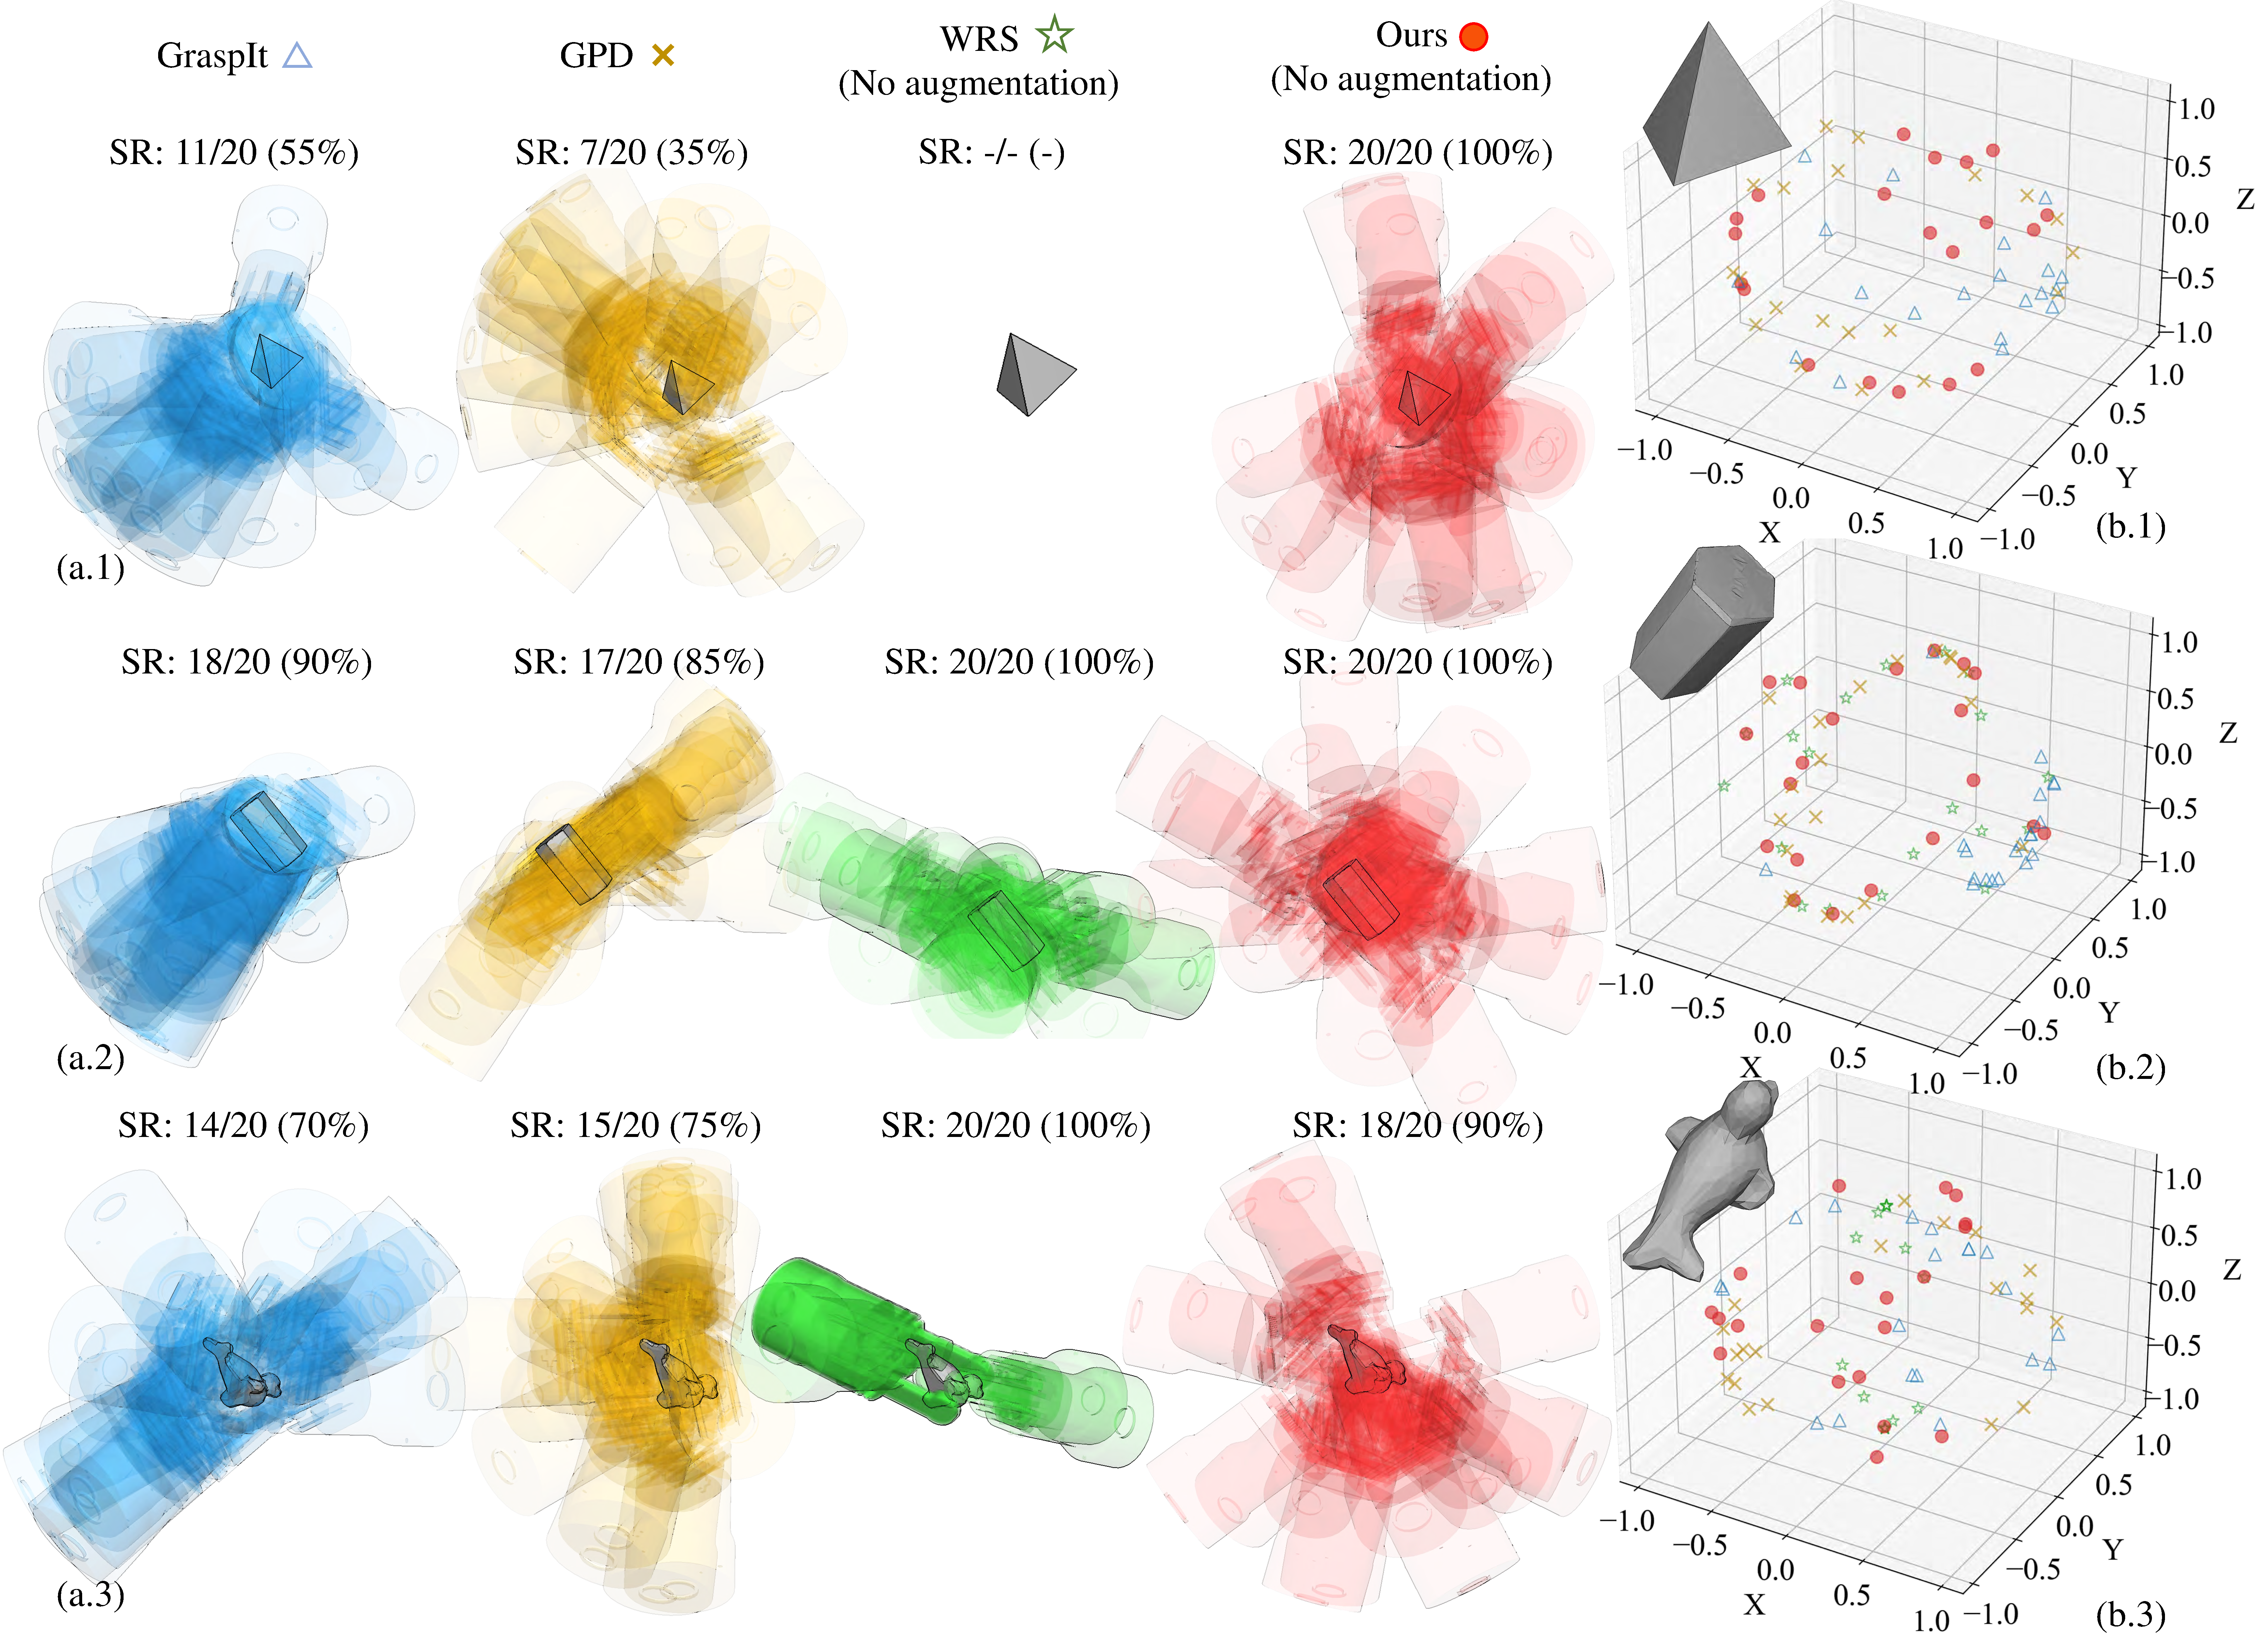
\includegraphics[width=1.0\linewidth]{FBGrasp/grasp_distribution_main.pdf}
    \caption{抓取分布可视化对比。(a) 各方法生成的抓取位姿展示（蓝色：GraspIt，黄色：GPD，绿色：WRS，红色：本文方法）；(b) 抓取构型在 3D 空间中的分布散点图。}
    \label{exp:distribution}
\end{figure}

\section{抓取成功率对比}
\label{sec:success_rate}

\subsection{实验设置与流程}
真实抓取实验在 ABB GOFA-5 平台上进行。为减少桌面碰撞并提升可达性，物体放置于细支撑柱上。运动规划采用 RRT-connect，任务流程为“接近、抓取、搬运到目标位”。为隔离视觉系统影响，实验中物体位姿均设为已知。

每个物体对每种方法执行 20 次抓取。若出现逆解不可达或碰撞，适当调整物体初始姿态以保证 20 个候选均可执行。成功标准为：物体被稳定提起并搬运，不发生滑落、脱落或明显姿态失稳。主要失败类型包括预接触碰撞、接触不足与构型不稳定。

\subsection{结果分析}
表 \ref{tab:statistical_results} 汇总了 9 个物体上的抓取成功率。本文方法平均成功率为 97.8\%，高于 WRS（76.7\%）、GPD（70.6\%）和 GraspIt（77.8\%）。

% 添加大表格：成功率对比
\begin{table*}[t]
    \centering
    \small
    \setlength{\tabcolsep}{4pt}
    \caption{各抓取规划方法的抓取成功率统计}
    \label{tab:statistical_results}
    \begin{threeparttable}
    \begin{tabular}{l|ccccccccc|c}
        \toprule
        \textbf{Method} & \textbf{四面体} & \textbf{巧克力} & \textbf{海豹} & \textbf{乐高} & \textbf{链轮} & \textbf{牛奶盒} & \textbf{杯面} & \textbf{电机座} & \textbf{齿轮} & \textbf{平均值} \\
        \midrule
        \textbf{Ours} & \textbf{100\%} & \textbf{100\%} & \textbf{90\%} & \textbf{100\%} & \textbf{100\%} & \textbf{95\%} & \textbf{95\%} & \textbf{100\%} & \textbf{100\%} & \textbf{97.8\%} \\
        WRS~\cite{wan2020planning} & 0\%   & 100\% & 100\% & 100\% & 95\%  & 95\% & 0\%  & 100\% & 100\% & 76.7\% \\
        GPD~\cite{ten2017grasp}& 35\%  & 85\%  & 75\%  & 85\%  & 85\%  & 70\% & 75\% & 70\%  & 55\%  & 70.6\% \\
        Graspit~\cite{miller_graspit_2021} & 55\%  & 90\%  & 70\%  & 90\%  & 80\%  & 80\% & 90\% & 75\%  & 70\%  & 77.8\% \\
        \bottomrule
    \end{tabular}
    \end{threeparttable}
\end{table*}

从单项结果看，WRS 在平行面物体上表现较好，但在四面体、杯面等缺少平行面的对象上无法生成有效抓取；GPD 与 GraspIt 可覆盖全部对象，但在锐边与复杂几何场景下成功率下降明显。本文方法对点、边、面接触统一建模，因此在四面体和齿轮等对象上仍保持较高成功率，体现了更好的几何适应性。

\section{本章小结}
\label{sec:summary}

本章通过分布统计与真实抓取测试验证了所提方法的有效性。仿真结果显示其抓取构型分布更广、更均匀；真实实验中平均成功率达到 97.8\%。

该方法目前仍是离线规划框架，依赖完整 3D 模型输入；同时主要面向平行夹爪，多指灵巧手场景仍需进一步扩展。尽管不同基线方法的参数调优机制不完全一致，实验结果仍能反映各方法在复杂几何接触条件下的能力差异。

\listoffigures                        % 插图索引
\listoftables                         % 表格索引

% 参考文献. 
% \bibliographystyle{gbt7714-numerical}
\bibliography{reference/refs}

\begin{publications}


{\heiti 一、论文}

[1] QIU M, HU Z, CHEN H, et al. Robotic grasp planning considering local concav-
ity of contact[C]//2025 IEEE International Conference on Robotics and Biomimetics
(ROBIO). 2025: 948-953.


{\heiti 三、专利}

[1] 张三. XXXXXXXXXXXXXXXXX: 202210050175. 8 [P]. 2022-10-14.


{\heiti 四、项目}

1. XX省“十五”制造业信息化工程重大科技攻关项目“基于支持智能化XXX设计的创新开发平台”（编号），主持，XXXX.XX.XX—XXXX.XX.XX。

2. XX省“十五”制造业信息化工程重大科技攻关项目“基于支持智能化XXX设计的创新开发平台”（编号），参与，第二， XXXX.XX.XX—XXXX.XX.XX。


\end{publications}
           % 发表论文清单
% 致谢
\begin{acknowledgement}
  时光荏苒，研究生阶段的学习与科研工作即将画上句号。在论文完成之际，谨向所有关心、帮助和支持过我的老师、同学、亲友致以最诚挚的感谢。

  首先，衷心感谢我的导师袁建军老师。袁老师为本课题提供了宝贵的实验资源与研究平台，并在课题方向把握、研究思路凝练以及学术规范养成等方面给予了我持续而细致的指导，使我受益匪浅。

  同时，感谢实验室各位指导老师的悉心帮助，特别感谢杜亮老师、鲍晟老师在科研训练和日常学习中给予我的指导与支持。尤其要特别感谢胡正涛老师，在论文撰写、实验分析和细节打磨过程中给予了我大量耐心、专业且富有启发性的指导，使论文得以不断完善。

  此外，衷心感谢南京大学张振宇老师、福建农林大学陈昊老师对本论文提出的宝贵指导与中肯建议。两位老师从不同视角提出了许多建设性意见，为论文内容的完善和研究深度的提升提供了重要帮助。

  感谢实验室的师兄师姐、师弟师妹们在科研与生活中的支持与帮助。与你们共同学习、讨论和合作的经历，让我在面对困难时始终能够获得力量，也让我度过了充实而难忘的研究生时光。

  最后，感谢我的家人和朋友长期以来的理解、包容与鼓励。正是你们无条件的支持，让我能够心无旁骛地投入学习和研究，并坚持走到今天。

  谨以此文，向所有给予我帮助的人致以诚挚谢意！

  \vspace{50bp}

  \hfill 作者署名：邱模聪

  \hfill 完成地点：上海大学

  \hfill 2026 年 4 月 1 日

\end{acknowledgement}
        % 致谢

\backmatter
\begin{appendix}
\chapter{经典函数公式}
论文中用到的经典函数公式如下。\\
\noindent{\bfseries (Sigmoid Function)}
Sigmoid 函数定义为
\[
\operatorname{Sigmoid}(x)=\frac{1}{1+e^{-x}}.
\]\\
\noindent{\bfseries (ReLU Function)}
ReLU 函数定义为
\[
\operatorname{ReLU}(x)=\max(0,x).
\]\\
\noindent{\bfseries (Leaky ReLU Function)}
Leaky ReLU 函数定义为
\[
\operatorname{LeakyReLU}(x)=\begin{cases}x,&x\geq0\\
\alpha x,&x<0\end{cases}
\]
其中 $\alpha$ 是一个较小的常数，通常取值为 0.01。\\

\chapter{用于定量比较的指标公式}
\label{cha:app_metrics}
章节~(\ref{sec:metrics}) 中提到的用于定量比较的指标公式如下。其中 $TP$、$TN$、$FP$ 和 $FN$ 分别表示真正例、真反例、假正例和假反例的数量。\\

\noindent{\bfseries (Precision)}
精确率定义为
\[
\text{Precision} = \frac{TP}{TP + FP}
\]
\noindent{\bfseries (Recall)}
召回率定义为
\[
\text{Recall} = \frac{TP}{TP + FN}
\]

\noindent{\bfseries (F1 Score)}
F1 分数定义为
\[
\text{F1 Score} = 2 \times \frac{\text{Precision} \times \text{Recall}}{\text{Precision} + \text{Recall}}
\]
\noindent{\bfseries (Matthews Correlation Coefficient)}
马修斯相关系数定义为
\[
\text{MCC} = \frac{TP \times TN - FP \times FN}{\sqrt{(TP + FP)(TP + FN)(TN + FP)(TN + FN)}}
\]
\noindent{\bfseries (Intersection over Union)}
交并比定义为
\[
\text{IoU} = \frac{TP}{TP + FP + FN}
\]
\noindent{\bfseries (Accuracy)}
准确率定义为
\[
\text{Accuracy} = \frac{TP + TN}{TP + TN + FP + FN}
\]

\chapter{\textrm{NECDNet} 额外检测结果}
\label{cha:app_necdnet_results}
\begin{figure}[!htbp]
    \centering
    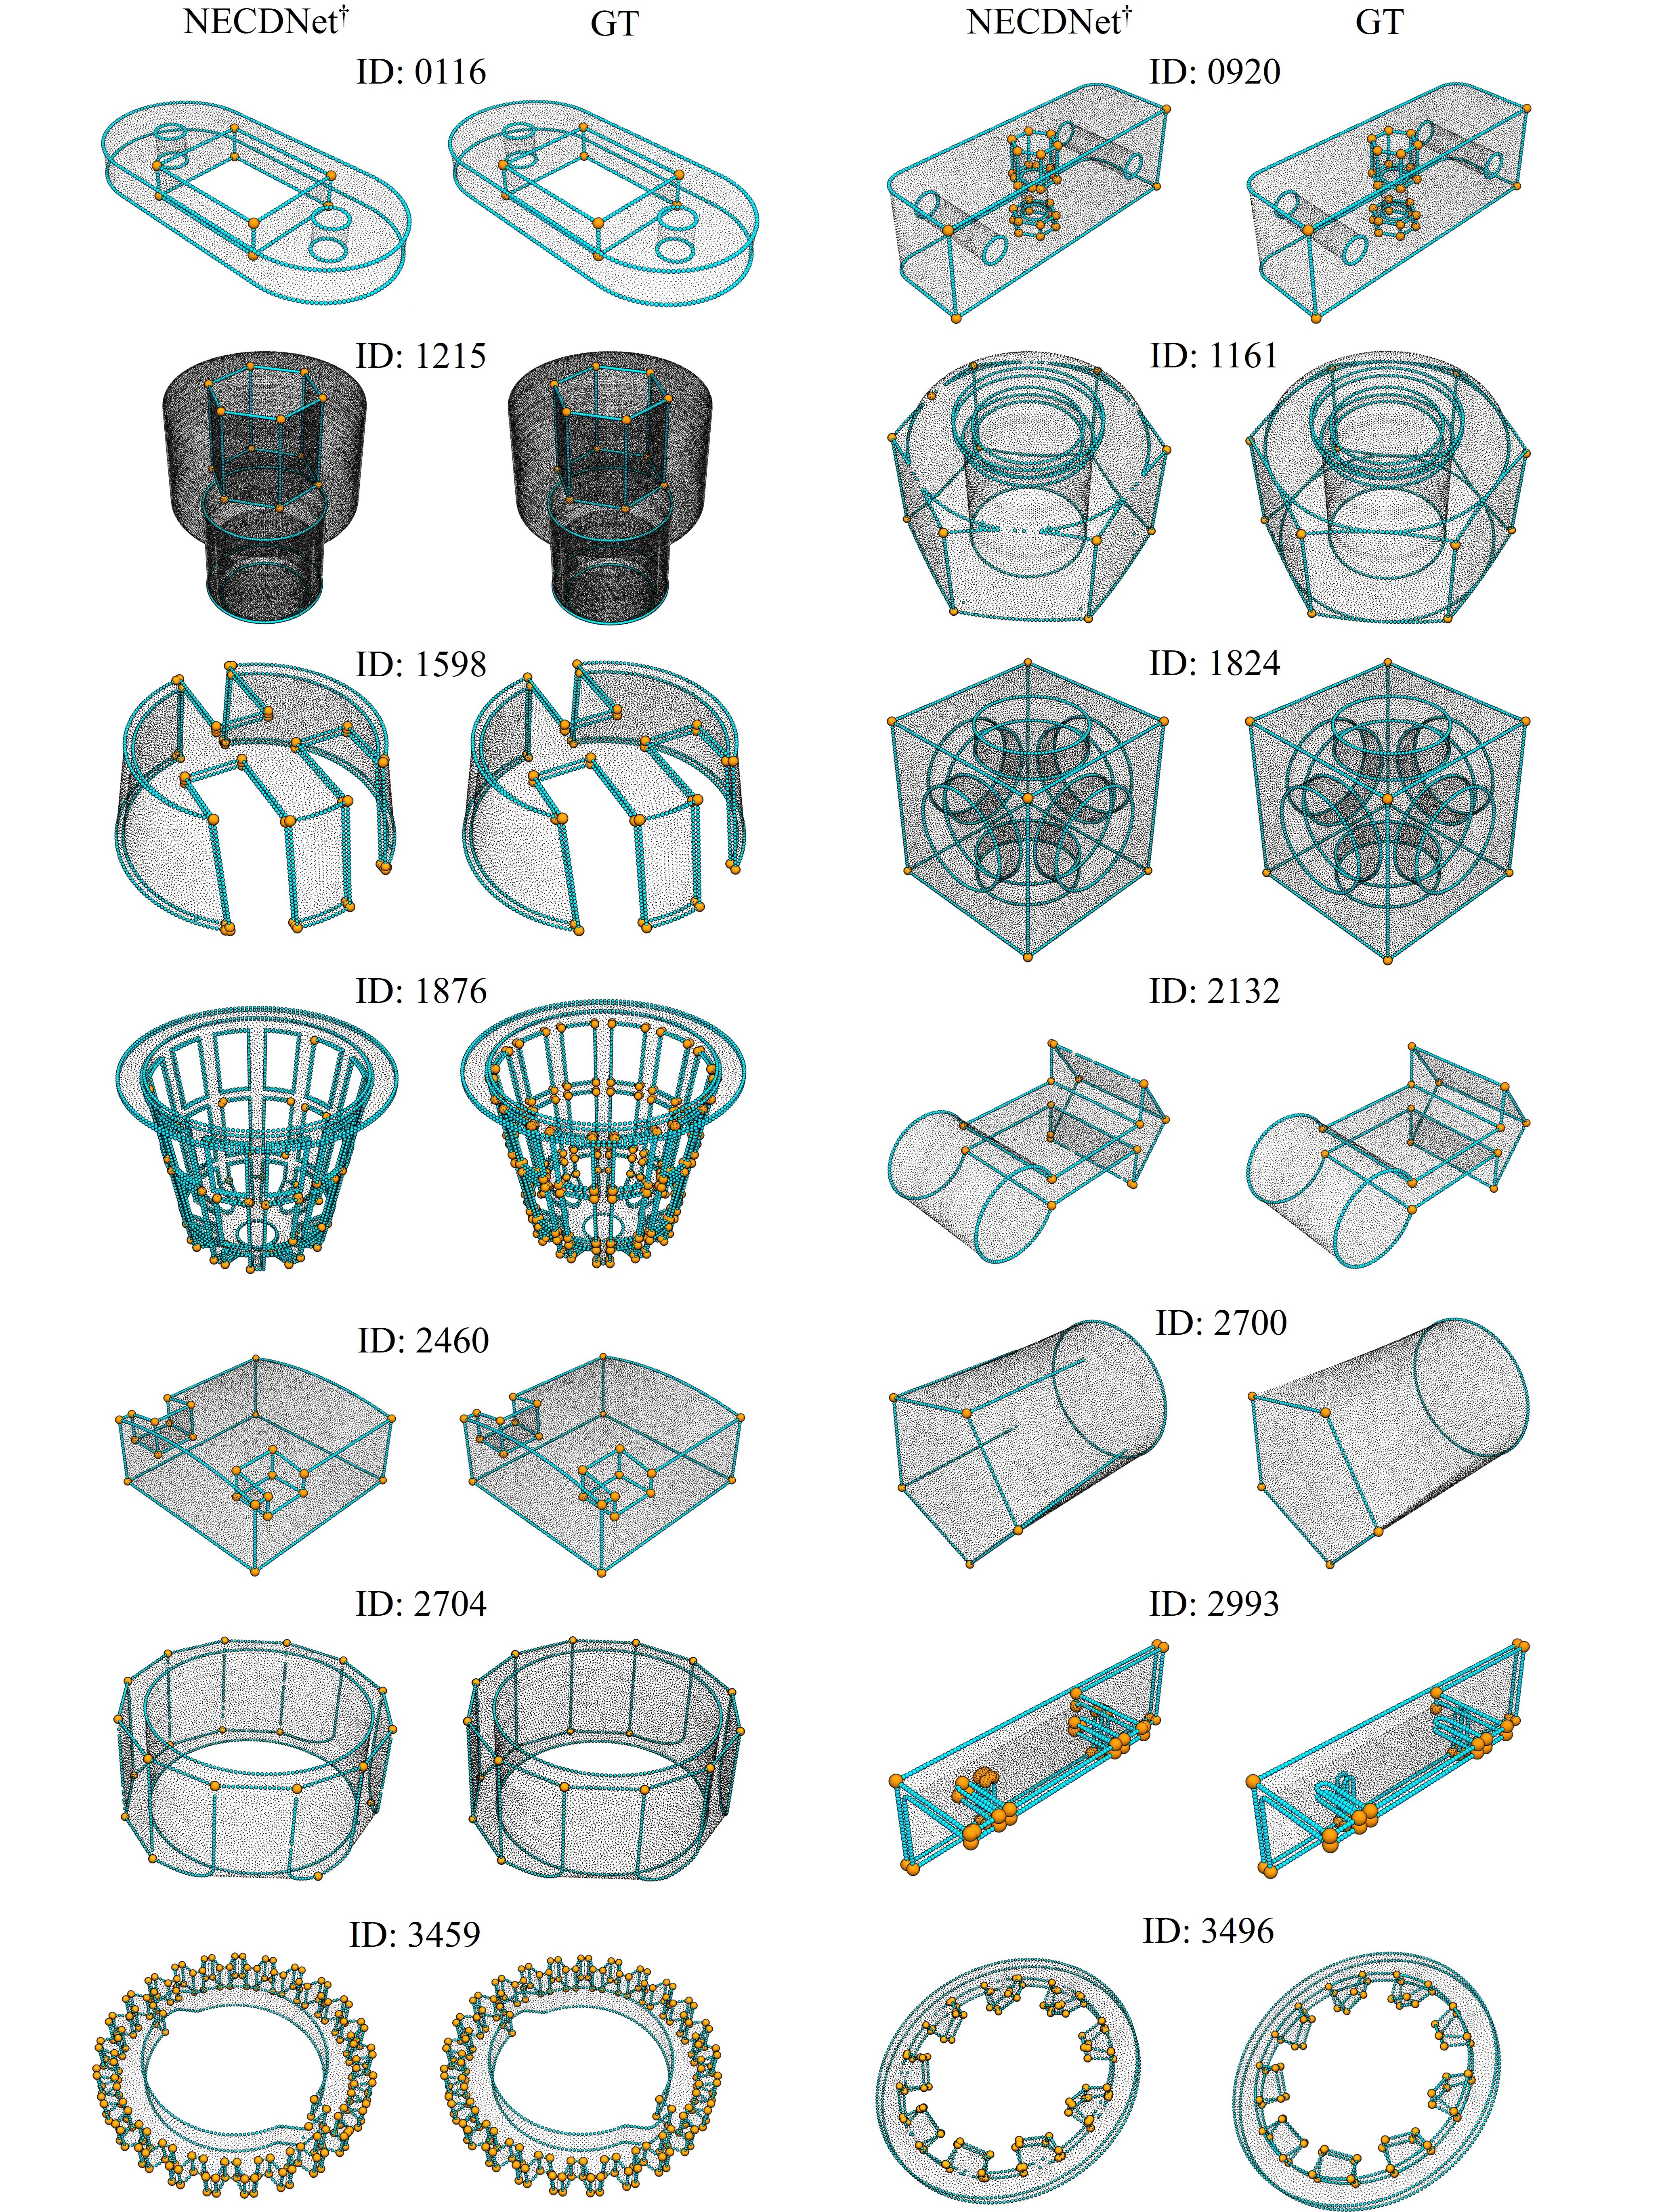
\includegraphics[width=0.95\textwidth]{NECDNet/additional_result.jpg}
    % \bicaption{NECDNet 在 ABC-Corner 数据集上的额外检测结果示例}{Additional detection results of NECDNet on the ABC-Corner dataset.}
    \label{fig:appendix_necdnet_results}
\end{figure}

\chapter{额外测试物体上的抓取构型分布图}

\begin{figure}[!htbp]
    \centering
    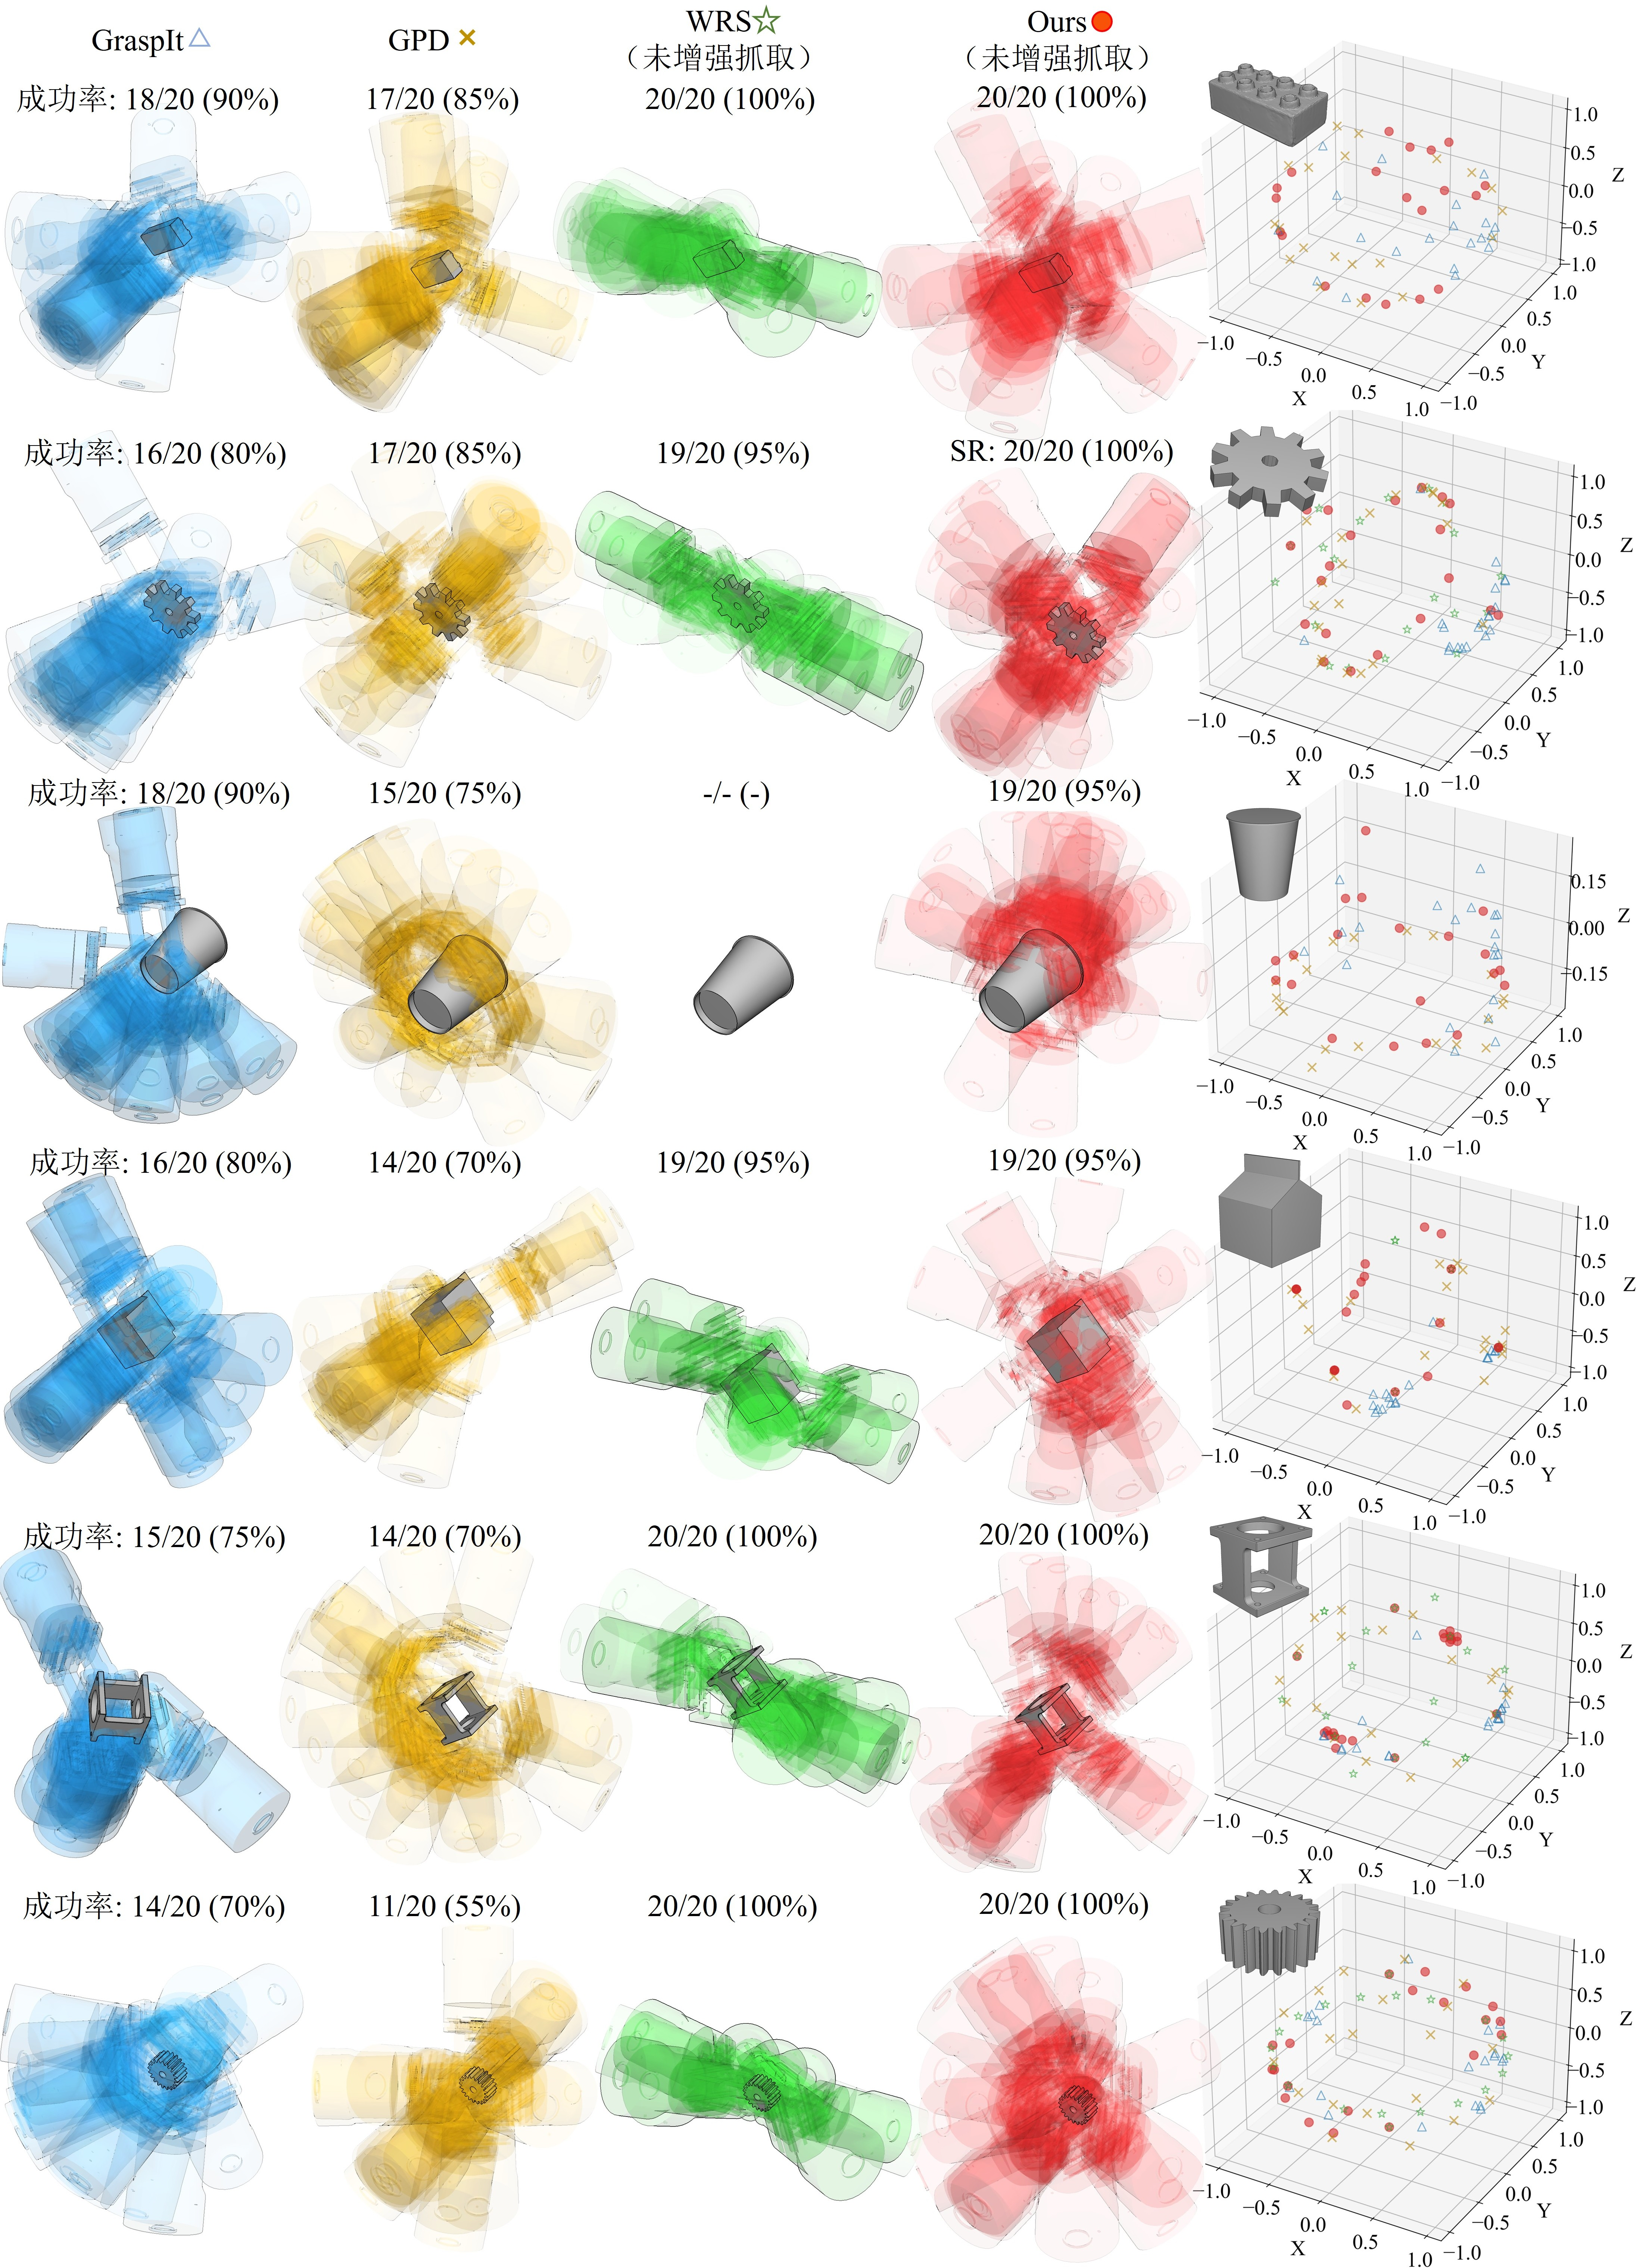
\includegraphics[width=0.95\textwidth]{FBGrasp/grasp_distribution.jpg}
    % \bicaption{在其余 7 种测试物体上的抓取构型分布图}{Grasp configuration distribution on the remaining 7 test objects.}
    \label{fig:appendix_grasp_distribution}
\end{figure}


\end{appendix}

\end{document}
